\documentclass[twoside]{scrartcl}

\usepackage[bluelinks]{drangreport}
% \usepackage[caecilia]{drangreport}

\usepackage{pgfplots}
\setcounter{section}{-1}
\usepgfplotslibrary{fillbetween}


%\renewcommand*\rmdefault{cmss}

%\usepackage{cmbright}

%%%%%%%%%%%%%%%%%%%%%%%%%%%%%%%%%%%%
%Messy stuff for plotting 
\newcommand{\vasymptote}[2][]{
    \draw [densely dashed,#1] ({rel axis cs:0,0} -| {axis cs:#2,0}) -- ({rel axis cs:0,1} -| {axis cs:#2,0});
}

\newcommand{\hasymptote}[2][]{
    \draw [densely dashed,#1] ({rel axis cs:0,0} -| {axis cs:0,#2}) -- ({rel axis cs:1,0} -| {axis cs:0,#2});
}

\newcommand*{\permcomb}[4][0mu]{{{}^{#3}\mkern#1#2_{#4}}}
\newcommand*{\perm}[1][-3mu]{\permcomb[#1]{P}}
\newcommand*{\comb}[1][-1mu]{\permcomb[#1]{C}}

\usepackage{pstricks}
\usepackage{pst-func}
\usepackage{pst-plot}

%%%%%%%%%%%%%%%%%%%%%%%%%%%%%%%%


\title{Methods I}

\usepackage[normalem]{ulem}
\usepackage{mathdots}



\hypersetup{pdfinfo={
Title={Mathematical Methods I Lecture Notes},
Author={Karim Bacchus},
Keywords ={Mathematical Methods I, M1M1, Lecture Notes, Imperial College, Maths},
}}


\begin{document}

\NotesTitle{1st}{Autumn 2014}{Mathematical Methods I}{Prof.~J.}{Mestel}
{

\section*{Syllabus}
\textit{The course supplies a firm grounding to A-level topics such as differentiation, integration, complex numbers and series expansions.}

\subsubsektion{Functions}\vspace*{-5pt}
Polynomial, rational, exponential, logarithmic, trigonometric and hyperbolic functions. Odd, even and inverse functions.

\subsubsektion{Limits}\vspace*{-5pt}
 Basic properties and evaluation. Continuity \& discontinuous functions.

\subsubsektion{Differentiation}\vspace*{-5pt}
 First principles, differentiability; logarithmic and implicit differentiation; higher derivatives; Leibniz's formula; stationary points and points of inflexion; curve sketching; parametric representation, polar co-ordinates.
 
\subsubsektion{Power Series}\vspace*{-5pt}
  The Mean Value Theorem. Taylor's Theorem with remainder. Infinite power series, radius of convergence. Ratio test; Taylor and Maclaurin Series. De l'Hopital's rule.
 
\subsubsektion{Integration}\vspace*{-5pt}
   Definition as Riemann limit; indefinite \& definite integrals; the fundamental theorem of calculus; integration by substitution and by parts; partial fractions; Existence of improper and infinite integrals. Integrals over areas and volumes.
  
  
\subsubsektion{Complex Numbers}\vspace*{-5pt}
  Definition; the complex plane; standard and polar representation; de Moivre's Theorem; $\exp(z)$ and $\log(z)$

\subsubsektion{First order Differentiation Equations}\vspace*{-5pt}
  Separable, homogeneous and linear equations. Special cases. Linear higher order equations with constant coefficients,

Course content at \url{http://www.ma.ic.ac.uk/~ajm8/M1M1}\\

\subsection*{Appropriate books}

{\shortskip
G. Stephenson \emph{Mathematical Methods for Science Students}

E. Kreyszig \emph{Advanced Engineering Mathematics} 
}
}


%\listoftodos
\TableofContents



%!TEX root = linear-algebra.tex
\pagebreak
\setcounter{page}{5}
\section{Introduction}
 \lecturemarker{0}{ 10.10.2014}



\begin{example}
Consider the definiton of the exponential function: \vspace{-10pt}

\begin{align} \nonumber
\exp(x) &= 1 + x + \frac{1}{2}x^2 + \frac{1}{6}x^3 + \dots && \vspace*{5pt}\\\nonumber
&= \sum_{n=0}^{\infty} \frac{x^n}{n!} &&
\end{align}

So $e^{100} = 1 - 100 + \frac{1}{2}100^2 - \frac{1}{6}100^3 + \dots \approx 0$\\

\textit{Is this really true?}\\
Yes, but this is not obvious. The series converges (i.e. tends to an answer) for all $x$. We will see this later...
\end{example}\vspace*{5pt}

\begin{example}
$f = \dfrac{4}{3+\cos x}$\\

Can we write the power series $f = a_0 + a_1 x + a_2 x^2 + \dots = \sum a_n x^n?$ where $a_n$ are known constants?\\

Yes, we find (somehow) that $f = 1 + \frac{x^2}{8} + \frac{x^4}{192} + \dots$\\

Does this series converge? Using Maple to find the series and plotting $f - \sum_0^{200} a_n x^n$, we actually find that at $\pm 3.60$ish, the difference is non-zero and it fails to converge. This is (apparently) amazing evidence of the existence of the complex plane...
\end{example}\vspace*{5pt}

\begin{example}[Limits]

$\displaystyle{\lim_{x \to \infty} (\sin x) = ? }$, it is undefined.\\

$\displaystyle{\lim_{x \to \infty} \left(\dfrac{\sin x}{x}\right) }= 0 $, from the sandwich theorem as 0 is squeezed between $\frac{1}{x}$ and $-\frac{1}{x}$\\\\

$\displaystyle{\lim_{x \to \infty} \left(\dfrac{1}{x\sin x}\right) = ? }$, undefined once more, since whenever $x = n\pi$, the denominator is 0.\\\\

$\displaystyle{\lim_{n \to \infty} \left(\frac{\sin n}{n}\right) }$, $n \in \R$ is not at all obvious (depends on how well you can approximate $\pi$)
\end{example}\vspace*{5pt}

Clearly we have work to do....



%%%%%%%%%%%%%%%%%%%%
%Actual lectures

\pagebreak


\sektion{Functions}         
A function  \lecturemarker{1}{14.10.2014}
 takes an ``input'' and gives a \emph{unique} output: $f(x) : x \in \mathbb{R}.$ $f(x)$ is the output or function value at $x$. $f:\mathbb{R} \rightarrow \mathbb{R}$ (alternative notation: $f$ ``maps'' input $\in \mathbb{R}$ to output $\in \mathbb{R}$). $f$ may not be defined for all reals. A function \textit{should} be defined along with the \emph{domain} of values over which it applies, e.g.:
\[f(x) = \sqrt{x^2 -1}\text{ for } x \geq 1\]

\begin{definition}
	 $[a,b] \; \text{ means } \forall x : \; a \leq x \leq b, (a,b) \; \text{ means } \forall x : \; a < x < b$.
These are called \emph{closed} and \emph{open} intervals respectively. 

\end{definition}


So $x \geq 1$ could be written as $x \in [1,\infty)$. By convention $\infty$ is never a closed interval since it is not a real number.\\

\begin{definition}
We also define the \emph{range} of a function to be the set of possible values $f(x)$ as it takes values of the domain.
\end{definition}
So $f(x) = \sqrt{x^2 -1 }$ in $[1,\infty)$ has the \emph{range} $[0,\infty)$.\\

Note: $\sqrt{}$ is always positive conventionally, otherwise it maps to more than one value $\implies f$ is not a function. Hence $\sqrt{x^2} = |x|$, \textit{not necessarily $x$.}\\


\subsubsektion{How might we define functions?}

\begin{enumerate}
\item An explicit formula, e.g. $f(x) = x^2\sin(x)$
 
As the domain is not given, we assume it applies for all $x$ or all sensible $x$. 

e.g. $f(x) = \dfrac{x+2}{x-1} \qquad$ ``sensible'' here means $x \neq 1$\\

\item Split ranges, e.g.
\[f(x) = \begin{cases}
 x & \text{ if }  x > 1\\
 \sin(x^2) & \text{ if } 0 < x \leq 1\\
 e^x & \text{ if } x \leq 0
 \end{cases}\]
 
 
\item As a solution to an equation

e.g. $f'' + x^2f = 0, f(0) = 1, f'(0) = 0$ \textit{may} define a function
 
Similarly we could define $f(x) = \displaystyle{\int_0^x t^t \, \mathrm{d}t}$

(Note: we use a different letter for the \textit{dummy} variable, $t$)\\

\item In words

 e.g. $f(x) =$ ``the maximum amount by which $x$ exceeds an integer for $ n = 1,2,\dots 100$''

\item An implicit definition

 e.g. $f(x)$ given by $f(x) + \frac{1}{2}\sin[f(x)] = x$

(or $y + \sin y = x :$ we can't solve for $y$ in terms of $x$ easily) given $x$, not easy to calculate $f(x)$\\

\item As a limit

 e.g. $x^{x^{x^{\iddots}}}$ or more formally: $f_1 = x^x$, $f_{n+1} = x^{f_n}$ for $n \geq 1$

If this process tends to a limit as $n \to \infty$ we may have defined a function.
\end{enumerate}\vspace*{5pt}

... And so on. There are lots of ways of defining functions.\\

\emph{How many functions are there?}

It turns out it's (a very large...) infinity (see M1F, there are different sizes of ``infinities")

Most functions are \sout{horrible} horrendous.
Even ones which look nice can be nasty...\\



\begin{example} $f(x) = \begin{cases}
 \sin(\frac{1}{x}) & x \neq 0\\
 0 & x = 0
 \end{cases}$\\
 
 \end{example}

The graph crosses the $x$-axis an infinite number of times between $[0,n]$:

\begin{center}
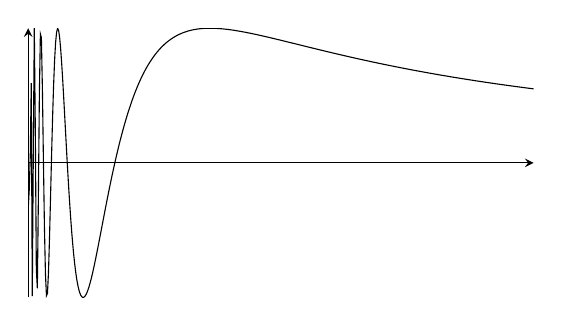
\begin{tikzpicture}
\begin{axis}[
axis lines=middle,
xtick = 0,
ytick = 0,
  width=8cm,height=5cm]
   \addplot[domain=0.0005:0.03,samples=500]{sin(1/x)};
 \end{axis}
\end{tikzpicture}
\end{center}

\begin{example} $f(x) = e^{-\frac{1}{x^2}}$


\begin{center}
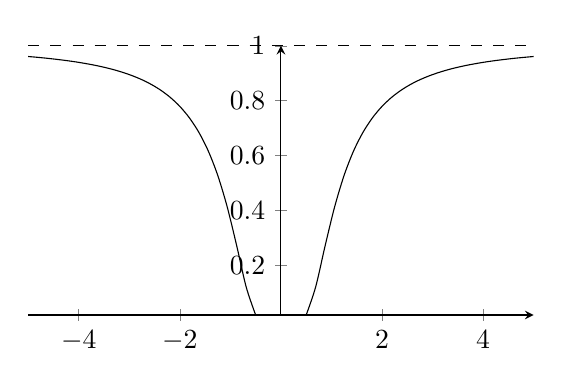
\begin{tikzpicture}
\begin{axis}[
%minor tick num=0,
axis y line=middle,
axis x line=middle,
domain=-5:5,
width=8cm,height=5cm
]
\addplot[domain=-5:-0.5,smooth]{exp(-1/x^2)};
\addplot[domain=0.5:5,smooth]{exp(-1/x^2)};
\addplot [dash pattern=on 4pt off 4pt] {1};
\end{axis}
\end{tikzpicture}
\end{center}

$f(x)$ is so flat at zero that the Macluarin (Taylor) Series converges to 0. This is NOT the right answer. We then call this a non-analytical function.
\end{example}\vspace*{5pt}


\begin{example} $f(x) = \displaystyle{\sum_{n=1}^{\infty} } \dfrac{\sin (n^4x)}{n^2} = \sin x + \dfrac{\sin 16x}{4} + \dfrac{\sin 81x}{9} + \dots$\\

This function is continous everywhere, differentiable nowhere.\\
\end{example}




\subsektion{Inverse functions} \lecturemarker{2}{16.10.2014}

Suppose we have a function $f$

%%%%%%%%%%%%%%%%%%%%%%
\begin{center}
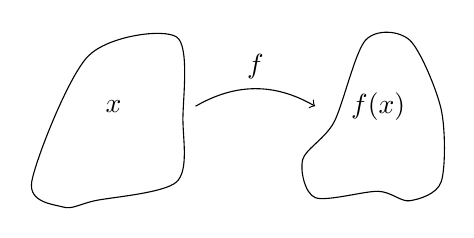
\begin{tikzpicture}[scale = 0.8]
\draw plot [smooth cycle] coordinates {(5,0.25) (6,0.35) (6.5, 0.2) (7,0.5) (7,1.65) (6.5,2.75) (5.8,2.75) (5.3,1.45) (4.8,0.85) } node at (6,1.7) {$f(x)$};
\path[->] (3.1,1.7) edge [bend left] node[above] {$f$} (5.0,1.7);
\draw plot [smooth cycle] coordinates {(1.0,.1)(1.5,.2)(2.8,.5)(2.9,1.5)(2.8,2.8)(1.4,2.5)(0.5,0.5)} node at (1.8,1.7) {$x$};
\end{tikzpicture}
\end{center}
%%%%%%%%%%%%%%%%%


\begin{definition}
If it is possible to find a function $g(f(x)) = x \quad \forall x$ in domain of $f$, then $g$ is called the \emph{inverse} of $f$. It's often denotes as $f^{-1}$.
\end{definition}

The domain of $f$ = the range of $f^{-1}$, and the range of $f$ = the domain of $f^{-1}$

\textit{Do inverses always exist?} 

Clearly not if ($\geq$) two $x$ values give the same value of $f(x) = y$ say. As we cannot determine a unique $x$ value given $y$. In practice, we try to solve $f(x) = y$ for $x$. This may find the inverse or tell us that there is a problem.\\


\begin{example} Find the inverse of $f(x) = \dfrac{x-1}{x+3} \qquad (x \neq 3)$
\[
\begin{aligned}
  y &= \dfrac{x-1}{x+3}\\[0.2cm]
  \implies y(x+3) &= x-1\\
  \implies x(y-1) &= -3y-1 \\[0.2cm]
  \implies x &= \dfrac{3y+1}{1-y} = f^{-1}(y)
\end{aligned}
\]



%%%%%%%%%%%%%%%%%%%%%%%%%%%%%%
\begin{center}
	

\begin{tikzpicture}
\begin{axis}[
minor tick num=0,
axis y line=middle,
axis x line=middle,
width=8cm,height=6cm]
\addplot[domain = -6:-3.8, smooth] {(x-1)/(x+3)};
\addplot[domain = -2.2:5, smooth] {(x-1)/(x+3)};
\vasymptote {-3};
\addplot [dash pattern=on 4pt off 4pt] {1};
\end{axis}
\end{tikzpicture}
\end{center}
The graph $y = f(x)$ helps us understand what is going on. So we sketch it, noting that $y = \frac{x-1}{x+3} = 1 - \frac{4}{x+3}$. For inverse to exist, all lines $y$ = constant must intersect $y = f(x)$ \sout{oncee} once and only once, which is clearly the case.

%%%%%%%%%%%%%%%%%%%%%%%%%%%%%%

%\tikz{
%\begin{axis}[
%minor tick num=1,
%ejes=-5:-1 -50:50,
%title={$y=f(x+1)=\dfrac{1}{x+1}$}
%]
%    \addplot {(x-1)/(x+3)};
%    \vasymptote {-3}
%    \draw [densely dashed] (axis cs:0,1) -- ({axis cs:0,1}-|{rel axis cs:1,0});
%\end{axis}}

\end{example}\vspace*{5pt}



\begin{example} Does $f^{-1}$ exist for $y = x + \frac{1}{x} = f(x)$?

Note that if $x = 2$, then $f(2) = 2.5$, but $f(\frac{1}{2}) = 2.5$ also...
maybe if we restrict the domain of $f$, we can find a sensible inverse. Lets try $y = x + \frac{1}{x}$
\[
\begin{aligned}
  \implies xy &= x^2 + 1\\
  \implies x^2 - xy + 1 &= 0\\
  \implies x &= \dfrac{y \pm \sqrt{y^2 -4}}{2}
\end{aligned}
\]


\emph{Which root should we take?}

Sketching $f(x)$, we can note that $y = k$ intersects the graph: 
\[\begin{cases}
\text{Not at all}& -2 < k< 2\\
\text{Once} & k = \pm 2\\
\text{Twice} & k>2 \text{ or } k<-2
\end{cases}\]



%%%%%%%%%%%%%%%%%%%%%%%%%%%%%%
\begin{center}
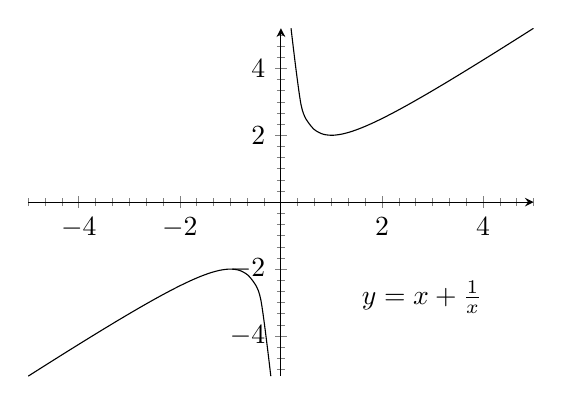
\begin{tikzpicture}
\begin{axis}[
minor tick num=5,
axis y line=middle,
axis x line=middle,
width=8cm,height=6cm
]
\addplot[domain = -5:-0.2, smooth] {x + 1/x};
\addplot[domain = 0.2:5, smooth] {x + 1/x};
\end{axis}
\node at (5,1) {$y = x + \frac{1}{x}$};
\end{tikzpicture}
\end{center}

%%%%%%%%%%%%%%%%%%%%%%%%%%%%%%


\vspace{5pt}

Suppose we restrict the domain of $f$ to be $|x| \leq 1$ (excluding $x=0$). Then we can define the inverse function:
\[f^{-1}(y) = 
\begin{cases}
 \dfrac{y - \sqrt{y^2 -4}}{2} & \text{ if } y \geq 2 \\[0.3cm]
 \dfrac{y + \sqrt{y^2 -4}}{2} & \text{ if } y \leq 2 
 \end{cases}
 \]
If instead we restrict the domain of $f$ to be $|x| \geq 1$ then:
\[f^{-1}(y) = \begin{cases}
 \dfrac{y + \sqrt{y^2 -4}}{2} & \text{ if } y \geq 2 \\[0.3cm]
 \dfrac{y - \sqrt{y^2 -4}}{2} & \text{ if } y \leq 2 \\
 \end{cases}
 \]
So a little care is required.
\end{example}

\subsubsektion{Trigonometric Functions}

\emph{Trigonometry:} 
% τρίγωνον 
trigōnon metron 
 - The Measuring of Triangles

Later we will define $\cos(x), \sin(x), \tan(x),$ but you already know them. 

\textbf{Inverse Cosine}

If $f(x) = \cos(x)$ then $f^{-1}(x) = \cos^{-1}(x)$ (or $\arccos(x)$) exists for some $x$ and some agreed domain of $f(x)$. 
  \begin{center}
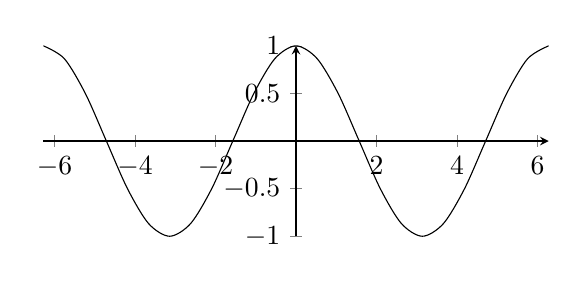
\begin{tikzpicture}
\begin{axis}[
minor tick num=0,
axis y line=middle,
axis x line=middle,
width=8cm,height=4cm
]
\addplot[domain =-6.28: 6.28,smooth] {cos(deg(x))};
\end{axis}
\end{tikzpicture}
\end{center}

The natural domain to restrict is $0 \leq x \leq \pi$. Then $\cos^{-1}(y)$ exists uniquely, provided $|y| \leq 1$. Now remove the restrictions on $x$. Solve the equation $\cos x = \alpha$:

General solution: $\boxed{ x = 2n\pi \pm \cos^{-1}\alpha \quad (n \in \Z)}$

But remember $0 \leq \cos^{-1} \leq \pi $ always!\\

\textbf{Inverse Sine}

  \begin{center}
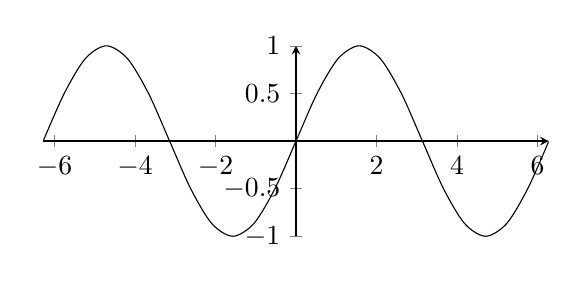
\begin{tikzpicture}
\begin{axis}[
minor tick num=0,
axis y line=middle,
axis x line=middle,
width=8cm,height=4cm
]
\addplot[domain =-6.28: 6.28,smooth] {sin(deg(x))};
\end{axis}
\end{tikzpicture}
\end{center}

We restrict $-\frac{\pi}{2} \leq x \leq \frac{\pi}{2}$ i.e. $|x| \leq \frac{\pi}{2}$. Then the inverse function $\sin^{-1}y$ exists, if $|y| \leq 1$. So $-\frac{\pi}{2} \leq \sin^{-1} \leq \frac{\pi}{2}$. Then the equation $\sin x = \beta$ has the general solution:
\[\begin{aligned}
x &= 2n\pi + \sin^{-1}\beta \mbox{ if $n$ is even}\\
x &= 2n\pi - \sin^{-1}\beta \mbox{ if $n$ is odd}\\
\implies \Aboxed{ x &= 2n\pi + (-1)^n \sin^{-1}\beta \quad (n \in \Z)}
\end{aligned}\]~

\textbf{Inverse Tan}\\
\begin{minipage}{7cm}


We restrict $-\frac{\pi}{2} \leq \tan^{-1}y \leq \frac{\pi}{2}$ defined $\forall y$.

So finally $tanx = \gamma$ has general solution: 
\[\boxed{x = n\pi + \tan^{-1}\gamma}\]
\end{minipage}
\begin{minipage}{7cm}
  \begin{center}
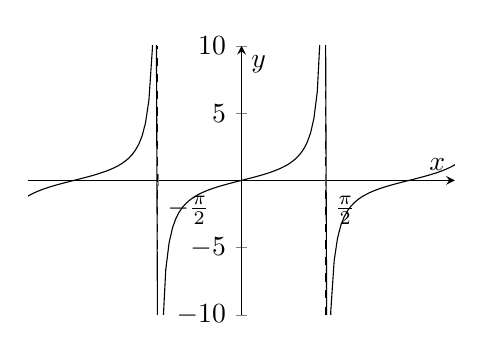
\begin{tikzpicture}
\begin{axis}
        [
    ymin=-10,ymax=10,
    xmin=-4,xmax=4,
    %clip=false,
    xtick=\empty,
    extra x ticks={-1.5708, 1.5708},
    extra x tick labels={$-\frac{\pi}{2}$, $\frac{\pi}{2}$},
    every extra x tick/.style={
            xticklabel style={anchor=north west},
            grid=major,
            major grid style={dashed,black}
    },
    axis lines = center,
    xlabel=$x$,ylabel=$y$,
    domain=-2*pi:2*pi,
    samples=200,
    width=7cm,height=5cm
    ]
    \addplot [black] {tan(deg(x))};
\end{axis}
\end{tikzpicture}
\end{center}
\end{minipage}

\pagebreak


\subsektion{Parity - Even \& Odd Functions} 
\vspace*{5pt}
\begin{definition} \lecturemarker{3}{ 17.10.2014}
A function $f(x)$ defined over a symmetric domain (i.e. $[-a,a]$) is called even $\iff f(-x) = f(x)$ and odd $\iff f(-x) = -f(x)$
\end{definition}

e.g. $x^2$ is even, $\sin x$ is odd. Functions need not be even or odd. But any function (over a symmetric domain) can be written as the sum of an even function \& an odd function. \\

\begin{example}
\[\dfrac{x}{x+1} = \dfrac{x}{x+1} \dfrac{(x-1)}{(x-1)} = \underbrace{\dfrac{x^2}{x^2-1}}_{\text{Even}} \;-\; \underbrace{\dfrac{x}{x^2-1}}_{\text{Odd}}\]
\end{example}

\begin{example}
\[\cos(x+3) = \underbrace{\cos x \cos 3}_{\text{Even}} \; - \; \underbrace{\sin x \sin 3}_{\text{Odd}}\]
\end{example}

In general, how do we write $f(x) = f_e(x) + f_o(x)$?
\begin{align*}
f(x) &= f_e(x) + f_o(x) \tag{1}\\ 
\implies f(-x) &= f_e(-x) + f_o(-x) \\
\implies f(-x) &= f_e(x) - f_o(x) \tag{2}
\end{align*}

Solving (1) and (2) by adding: 
\[\implies f_e(x) = \frac{1}{2} [f(x) + f(-x)]\]

Similarly \[f_o(x) = \frac{1}{2} [f(x) - f(-x)]\]

To prove that we can always find these two functions, start again from other way:

Define $f_e$ and $f_o$ as above, note: 
\begin{enumerate}
\item $f_e$ is even
\item $f_o$ is odd
\item $f_e + f_o = f$
\end{enumerate}

This proves that any $f$ has an even part and an odd part.\\

\begin{example}
Redo Example 1.6. $f(x) = \dfrac{x}{x+1} = f_e(x) + f_o(x)$

\[\begin{aligned}\implies f_e(x) &= \frac{1}{2} \left[\dfrac{x}{x+1} + \dfrac{-x}{1-x}\right]\\
&= \frac{1}{2} \left[\dfrac{x - x^2 - x^2 -x}{(1+x)(1-x)}\right] = \dfrac{-x^2}{1-x^2} = \dfrac{x^2}{x^2-1}\end{aligned}\]

\end{example}

\subsubsektion{Evaluating Integrals}
Parity is a great help when evaluating integrals.\\

What is $\displaystyle{ \int_{-\pi}^{\pi} \dfrac{x + \sin (x^3)}{1 + e^{x^2}} \, \mathrm{d}x}$?\\

Replacing $x$ by $-x$ we can see that the integrand is an odd function since $f(-x) = -f(x)$. Hence the Integral = 0.


  \begin{center}
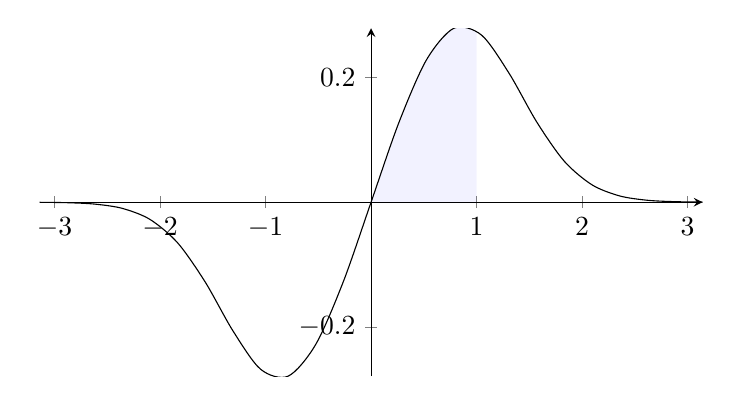
\begin{tikzpicture}
\begin{axis}[
minor tick num=0,
axis y line=middle,
axis x line=middle,
width=10cm,height=6cm
]
\addplot[name path=f, domain =-pi: pi,smooth] {(x + sin (x^3))/(1 + e^(x^2))};
     \path[name path=axis] (axis cs:0,0) -- (axis cs:1,0);

 \addplot [
        thick,
        color=blue,
        fill=blue, 
        fill opacity=0.05
    ]
    fill between[
        of=f and axis,
        soft clip={domain=0:1},
    ];
\end{axis}
\end{tikzpicture}
\end{center}\vspace*{5pt}

\begin{proposition} In general $I = \displaystyle{\boxed{\int_{-a}^{a} f_o(x) \, \mathrm{d}x = 0}}$\end{proposition}
\begin{proof}Substituting $t = -x$
\begin{align*}\nonumber
 \implies I &= \int_{a}^{-a} f_o(-t) \, (\mathrm{-d}x) \\
 &=  \int_{-a}^{a} f_o(-t) \, (\mathrm{d}x) \qquad \text{[Use - sign to swap limits]}\\
 &=  -I 
\end{align*}

Hence $I = -I \implies I = 0$. We conclude that if $f(x)$ is odd, then $ \displaystyle{\int_{-a}^{a} f(x) \, \mathrm{d}x = 0}.$\end{proof}

Later we will deal with power series $f(x) = a_0 + a_1x + a_2x^2 + ...$, where $a_i$ is a given constant  for $i \in \N$. 

If $f(x)$ is even then $a_1 = 0, a_3 = 0$ etc., i.e. $a_{odd} = 0$. If $f(x)$ is odd then $a_0 = 0, a_2 = 0$ etc., i.e. $a_{even} = 0$. So even/odd functions only have even/odd powers of $x$.\\


\subsektion{Periodicity}\vspace*{5pt}
\begin{definition} 
We say a function $f(x)$ is $T$-periodic if and only if $f(x + T) = f(x)~ \forall x$, where $T >0 $ and $T$ is the smallest value for which this holds.
\end{definition}


So although $\sin (x+ 4\pi) = \sin x \; \forall x$, we do not say that $\sin x$ is $4\pi$ periodic, as $\sin (x + 2\pi) = \sin (x) $ as well.\\

\bgroup
\def\arraystretch{1.5}
\begin{table}[H]
    \begin{tabular}{l|l}
    \hline
    $f(x)$            & period                                                    \\ \hline
    $\cos^2x$         & $\pi$                                                     \\
    $\cos |x|$        & $2\pi$                                                    \\
    $|\cos x|$        & $\pi$                                                     \\
    $\sin (\alpha x)$ & $\frac{2\pi}{\alpha} \quad (\alpha \neq 0)$               \\
    $3$                 & depends on definition, say period = 0 \& change definiton \\
    $\sin |x|$        & not periodic                                              \\
    $| \sin x|$       & $\pi$                                                     \\
    \end{tabular}
\end{table}
\egroup

\emph{Are there any other periodic functions (other than the trigonometric ones)?}\\

  \begin{center}
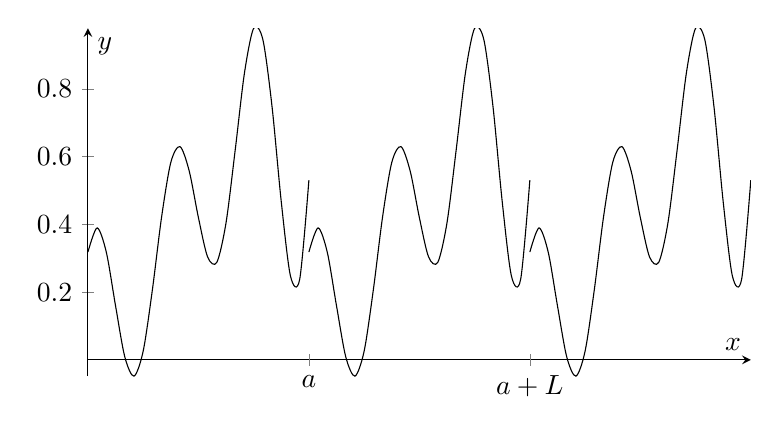
\begin{tikzpicture}
\begin{axis}
        [
    %ymin=-10,ymax=10,
    %xmin=-4,xmax=4,
    %clip=false,
    xtick=\empty,
    extra x ticks={100,200},
    extra x tick labels={$a$, $a+L$,},
    axis lines = center,
    xlabel=$x$,ylabel=$y$,
    width=10cm,height=6cm
    ]
    \addplot [domain = 0:100, smooth] {cos(x-120) + 0.5*cos(3*(x-120) + 0.23) + 0.5*cos(5*(x-120) - 0.4 ) + 0.5*cos(7*(x-120) + 2.09 ) + 0.5*cos(9*(x-120) - 3)+0.3};
    \addplot [domain = 100:200, smooth] {cos(x-220) + 0.5*cos(3*(x-220) + 0.23) + 0.5*cos(5*(x-220) - 0.4 ) + 0.5*cos(7*(x-220) + 2.09 ) + 0.5*cos(9*(x-220) - 3)+0.3};
    \addplot [domain = 200:300, smooth] {cos(x-320) + 0.5*cos(3*(x-320) + 0.23) + 0.5*cos(5*(x-320) - 0.4 ) + 0.5*cos(7*(x-320) + 2.09 ) + 0.5*cos(9*(x-320) - 3)+0.3};
\end{axis}
\end{tikzpicture}
\end{center}


%%%%%%%%%%%%%%%%%%%%%%
%%%% 
%%%% Sketch of Random function a to a+L
%%%%
%%%%%%%%%%%%%%%%%%%%%%

We can turn any function into a periodic one. Any function defined on a finite interval can be extended into a periodic function over all $\R$ by copying. Define $f(x + L) = f(x)$ to replicate the behaviour $\forall x$.\\


\subsektion{Polynomials}
\vspace*{5pt}
\begin{definition}
An $n$th order  \lecturemarker{4}{21.10.2014} polynomial in $x$ is a function of the form: \[f(x) = \displaystyle{\sum_{a=0}^{N} a_n x^n}\]
 where $a_N \neq 0$. $N$ is called the \emph{degree} or \emph{order} of the polynomial.. $a_n$ for $n = 0,...,N$ are called the coefficients. If $a_n$ is real $\forall n$, we say the polynomial is real (even if $x$ may be complex).
\end{definition}

\begin{theorem}[The Fundamental Theorem of Algebra]

Every polynomial has a root (possibly complex). In general, we call a value $\alpha$ a root of $f(x)$ if $f(\alpha)$ = 0. 

\end{theorem}

\textit{Proof.} See next year's course \textsc{M2PM3 Complex Analysis.}\\


\begin{corollary}
If $c$ is a root of an $N$th order polynomial $P_N(x)$, then we can write $P_N(x) = (x-c)P_{N-1}(x)$.
\end{corollary}\vspace*{5pt}

\begin{corollary}
Every $N$th order polynomial has precisely $N$ roots, allowing for repeated roots. e.g. $(x-1)^2$ has roots 1,1.
\end{corollary}\vspace*{5pt}

\begin{corollary}
If $P(x)$ is a real polynomial with a complex root $\alpha + i\beta$ ($\alpha, \beta$ real, $\beta \neq 0$), then it also has root $\alpha - i\beta$ (the complex conjugate).
\end{corollary}\vspace*{5pt}

\begin{corollary}
Every real polynomial can be written as:\\ $P_N(x) = A(x-r_1)(x-r_2)...(x-r_M)((x-\alpha _1)^2 + \beta ^2)((x-\alpha _2)^2 + \beta _2^2)...((x - \alpha _ L)^2 + \beta _L^2)$

Where $r_1.. r_M$ are the real roots, and $(\alpha \pm i \beta),... (\alpha _L \pm i\beta _L)$ are the complex roots and $M + 2L = N$
\end{corollary}

i.e. Any real polynomial can be written as a product of real linear and quadratic factors.

N.B. If the polynomial is not real (i.e. if at least one coefficient is strictly complex), then the complex roots need not be in conjugate pairs.\\


\subsubsektion{Roots of polynomials}
\begin{itemize}

\item Linear: $ax + b = 0$, one trivial root

\item Quadratic: $ax^2 + bx + c = 0$\\

Formula: $x = \dfrac{-b \pm \sqrt{b^2 - 4ac}}{2a} \quad$ \underline{OR} $\quad x = \dfrac{2c}{-b \pm \sqrt{b^2 - 4ac}}$\\


\emph{Exercise 1}: Show these are the same. 

\emph{Exercise 2}: Use your calculator to solve the equation $\epsilon x^2 + (1 + \epsilon)x + 1 = 0$, where $\epsilon$ is very small (i.e. $10^{-12}$).

Subtracting two numbers which are very close together leads to severe accuracy loss c.f. Patriot missiles. The ``Best'' formula to solving a quadratic depends on $a, b$ and $c$ in practice.

\item Cubics: $ax^3 + bx^2 + cx + d = 0$

There is a formula\footnote{\tiny $x = \sqrt[3]{\left(\frac{-b^3}{27a^3} + \frac{bc}{6a^2} - \frac{d}{2a}\right) + \sqrt{\left(\frac{-b^3}{27a^3} + \frac{bc}{6a^2}-\frac{d}{2a}\right)^2 - \left(\frac{c}{3a}-\frac{b^2}{9a^2}\right)^3}} + \sqrt[3]{\left(\frac{-b^3}{27a^3}+\frac{bc}{6a^2}-\frac{d}{2a}\right) + \sqrt{\left(\frac{-b^3}{27a^3}+\frac{bc}{6a^2}-\frac{d}{2a}\right)^2 - \left(\frac{c}{3a}-\frac{b^2}{9a^2}\right)^3}} - \frac{b}{3a}$\\},
 but it has very little practical use.\\

\item Quartics: $ax^4 + bx^3 + cx^2 + dx + e = 0$

There is also a general formula... once again not worth knowing\footnote{or even typesetting...}\\

\item Quintics: $ax^5 + bx^4 + cx^3 + dx^2 + ex + f = 0$

There is no general formula to express the roots in terms of radicals. See \textsc{M3P11 - Galois Theory} in 3rd year. But one can easily find the roots in practice for any particular case.\\

\item $N > 5$: Similarly no formula. However considering general $N$:
\begin{align*} \nonumber
P_N(x) &= a_Nx^N + a_{N-1}x^{N-1} + \dots\\ 
&= a_Nx^N\left[1 + \frac{a_{N-1}}{a_N} \frac{1}{x} + \frac{a_{N-2}}{a_N} \frac{1}{x^2} + \dots \right]
\end{align*}


As $\displaystyle{ |x| \to \infty, \frac{1}{x^N} \to 0 }$, So for large $|x|, P_N \approx a_Nx^N$. 

Hence if $a_N > 0$ WLOG, then as $\displaystyle{x \to \pm \infty , \; P_{2N}(x) \to +\infty \text{ and } P_{2N+1} \to \pm \infty }$\\  
%%%%%%%%%%%%%%%%%%
%
% PUT SKETCH OF POINT HERE

%%%%%%%%%%%%%%%%%
\end{itemize}

\subsektion{Rational Functions}\vspace*{5pt}

\begin{definition}A function  \lecturemarker{5}{23.10.2014} of the form $f(x) = \dfrac{P(x)}{Q(x)}$, where $P(x)$ and $Q(x)$ are polynomials is called a \emph{rational function}.
\end{definition}

We \textit{could} require that the order of $P < $ order of $Q$. If this doesn't happen, we can use polynomial division to write: 

\[\frac{P}{Q} = R(x) + \frac{S(x)}{Q(x)} \quad \text{ where } R \text{ and } S \text{ are also polynomial}\]\vspace*{5pt}

\begin{example}
\[\begin{aligned}
\frac{x^2 + x}{x -1} &= \frac{x^2 - x + 2x}{x-1}\\
&= x + \frac{2x}{x-1}\\
&= x + \frac{2x-2+2}{x-1}\\
&= (x+2) + \frac{2}{x-1} \end{aligned} \]
\end{example}
We could also require that $P$ and $Q$ have no common factors i.e. $\nexists \alpha : P(\alpha) = 0 = Q(\alpha)$ 

Let's do this! (for simplicity). Any zero of $Q(x)$ is then a \emph{singularity} or \emph{pole} or infinity of $\frac{P}{Q}$ and is important. This behaviour is illustrated by...\\


\subsubsektion{Partial Fraction Decomposition}

Suppose $Q$ has degree $N$, with no repeated root, i.e.
\[Q = \lambda (x-r_1)(x-r_2)\dots(x-r_N)\] 
Where $\lambda \neq 0, r_i \neq r=j$ unless $i = j$ and $r_i \in \mathbb{C}$

Then we can write:
\[\frac{P}{Q} = \frac{A_1}{x-r_1} + \frac{A_2}{x-r_2} + \dots + \frac{A_N}{x-r_N} + \overbrace{R(x)}^\text{if needed} \]\vspace*{5pt}

We can easily find $A_i$ by multiplying through $Q$:\vspace*{5pt}
\begin{align} \nonumber P &= \frac{A_1Q}{x-r_1} + \frac{A_2Q}{x-r_2} + \dots + \frac{A_NQ}{x-r_N}\\ \nonumber
&= A_1 \lambda(x-r_2)(x-r_3)\dots(x-r_N) + \frac{A_2Q}{x-r_2} + \dots + \frac{A_NQ}{x-r_N}  \tag{$*$}
\end{align}

Putting $x = r_1$ into $(*)$; $Q(r_1) = 0$, so:\vspace*{5pt}
\[P(r_1) = A_1 \lambda (r_1 - r_2)(r_1 - r_3)\dots(r_1 - r_N) \]

Using the product rule for differentiation, we also now have:
\[
Q'(x) = \lambda[(x-r_2)\dots(x-r_N)] + \lambda(x-r_1)[\text{ a load of stuff }]
\]

So \[Q'(r_1) = \lambda(r_1-r_2)(r_1-r_3)\dots(r_1-r_N)\] 

hence $P(r_1) = A_1Q'(r_1)$ or $A_1 = \dfrac{P(r_1)}{Q'(r_1)}$

So obviously \[\boxed{A_i = \dfrac{P(r_i)}{Q'(r_i)} \quad i = 1,2,...,N}\]\vspace*{5pt}

\emph{What could go wrong?}

\begin{itemize}
\item[(a)] \textit{What if (some of) the roots are complex?}\\
Algebra still works. But for some purposes we may prefer to keep things real.
 \begin{align*} \nonumber \text{e.g.}\quad \frac{3}{x^3+1} = \frac{3}{(x+1)(x^2 - x + 1)} &= \frac{3}{(x+1)(x-\omega)(x+\omega *)} \\ &= \frac{A_1}{x+1} + \frac{A_2}{x - \omega} + \frac{A_3}{x - \omega *}
 \end{align*}\vspace*{5pt}

Using the formula we obtained for $A_i$, we get $A_1 = 1, A_2 = -\omega, A_3 = -\omega *$
\begin{align} \nonumber \frac{3}{x^3 + 1} &= \frac{1}{x+1} - \frac{\omega}{x-\omega} - \frac{\omega *}{x - \omega *} \\\vspace*{5pt} \nonumber
&= \frac{1}{x+1}  - \frac{x-2}{x^2 - x + 1} \end{align}

Alternative Partial Fraction Form for real polynomials:
\[\frac{P}{Q} = R + \frac{A_1}{(x-r_1)} + \dots + \underbrace{\frac{Cx + D}{Cx^2 + \delta x + \delta}}_\text{for complex roots} + \dots \]

\item[(b)] \textit{What if there are repeated roots?}

e.g. 
\[Q(x) = \lambda(x-r_1)^2(x-r_3)(x-r_4)\dots(x-r_N)\]

Then 
\[\frac{P}{Q} = R + \frac{A_1}{(x-r_1)^2} + \frac{B}{(x-r_1)} + \frac{A_3}{(x-r_3)} + \dots + \frac{A_N}{(x-r_N)}\]

Sometimes it's easiest to manipulate the numerator:\\
\end{itemize}

\begin{example}
\[	\frac{x}{(x+2)^2(x+3)}\]
	
\emph{Example cancelled due to laziness of lecturer.}
\end{example}\vspace*{5pt}

\subsubsektion{Use of Partial Fractions} 

Calculus and curve plotting. Every rational function can be integrated in terms of simple functions. Also useful when differentiating many times:\\

\begin{example}
\[f = \frac{x+3}{x^2 + 4x + 3}\]

We have $P = x+1$, $Q'=  2x+4$, so $A_1 = \frac{-1}{-2}$, $A_2 = \frac{1}{2}$: 
	\[
\begin{aligned}
 f &= \frac{\frac{-1}{-2}}{x+3} + \frac{\frac{1}{2}}{x+1}\\
  &= \frac{1}{2}\left[\frac{1}{x+3} + \frac{1}{x+1}\right]
\end{aligned}
\]

So differentiating: 

\[
\begin{aligned}
  f' &= \frac{1}{2}\left(-\frac{1}{(x+3)^2} - \frac{1}{(x+1)^2}\right)\\
  f'' &= \frac{1}{2}\left(\frac{2}{(x+3)^3} + \frac{2}{(x+1)^3}\right)\\
  f^{(n)} &= \frac{1}{2}\left[\frac{1}{(x+3)^{n+1}} + \frac{1}{(x+1)^{n+1}}\right](-1)^nn!
\end{aligned}
\]


\end{example}


\pagebreak



\sektion{Infinite Series}\vspace*{5pt}

\begin{definition}An \emph{infinite series} is a \lecturemarker{6}{24.10.2014} function of the form $f(x) = \sum_{n=0}^{\infty} a_n x^n$\end{definition}

We will assume for now that the infinite sum converges (i.e. tends to a limit) for at least some values of $x$. We will also assume we can manipulate infinite series sensibly. The $a_n$ are called coefficients (may be $\in \mathbb{C}$)

\subsektion{The Exponential Function}

\[f(x) = \sum_{n=0}^{\infty} \frac{x^n}{n!} = 1 + x + \frac{x^2}{2} + \frac{x^3}{6} + \dots\]

In fact this series converges $\forall x$.

Forget everything we know about $e^x$ for now... \emph{What can we deduce about $f(x)$?}

If $x>0, f(x) > 1$ by inspection, and also $x$ increases as $f(x)$ increases. Question 6 on the problem sheets proved that $\forall x,y, f(x)f(y) = f(x+y)$. 

Setting $y = -x$, yields $f(-x) = \frac{1}{f(x)}$, which tells us about when $ 0<x <1$. $f(x) \to 0$, as $x \to -\infty$ etc. It follows that $f(x)$ has an inverse function $g(x)$ whose domain is $(0,\infty)$ and range $(-\infty,\infty)$, so we know that $x = g(f(x)) \, \forall x$ and $x = f(g(x)) \, x>0$.\\

Now consider 
\[
\begin{aligned}
  x^2 = x.x &= f(g(x)\cdot f(g(x))\\
  &= f(g(x) + g(x)) \quad \mbox{ [By $f(x)f(y) = f(x+y)$]}\\
  &= f(2g(x))
\end{aligned}
\]
Clearly induction $x^n = f(ng(x))$ for $n \in \N$\\

\begin{definition} 
$x^{\alpha} = f(\alpha g(x)) = e^{\alpha \log x}$ for $x >0,$ any arbitrary $\alpha$

$a^x = f(x(g(a))$ for $a > 0$, any arbitrary $x$
\end{definition}


From the definiton of $f$, $a^x = 1 + x(g(a)) + \frac{1}{2} [xg(a)]^2 + \frac{1}{3!}[xg(a)]^3 + \dots$

Choose $a$ such that $g(a) = 1$, then we have:
\[a^x = 1 + 1 + \frac{1}{2} + \frac{1}{3!} + \dots = 2.718281828459...\]

Let's call this value (...wait for it), $e$

 Then $g(e) = 1$, so 
 \[e^x = \sum_{n=0}^{\infty} \frac{x^n}{n!} = 1 + x + \frac{x^2}{2} + \frac{x^3}{6} + \dots \]

From now we can use all the properties of the exponential function,

 e.g. $e^xe^y = e^{x+y}, \quad (e^a)^b = e^{ab}, \quad e^0 = 1$. 

Calling $g(x) = \log(x) = ln(x)$, we have the usual properties which follows from the first problem sheet:\\
\begin{itemize}
\item $\log(uv) = \log(u) + \log(v)$
\item $\log(1) = 0$
\item ``$\log(0)= -\infty$''
\item $\log (\frac{u}{v}) = \log(u) - \log(v)$
\item $\log(a^b) = b\log a$
\item $a^b = e^{b \log a}$
\end{itemize}
(We will not consider logarithms to different bases)\\

$e^x$ is defined $x \in R$, \emph{ what if $x$ is complex or purely imaginary?}\vspace*{5pt}

\begin{definition}
Write $x = i\theta, \theta \in R$, then define $e^{i\theta}$ to be:
\[\begin{aligned}f(i \theta) &= \sum_{n=0}^{\infty} \frac{(i\theta)^n}{n!}\\
&= 1 + i\theta + \frac{1}{2}(i\theta)^2 + \frac{1}{3!}(i\theta)^3 + \frac{1}{4!}(i\theta)^4 + \dots\\
& = \left(1 - \frac{1}{2}\theta^2 + \frac{\theta^4}{4!} - \frac{\theta^6}{6!} + \dots\right) + i\left(\theta - \frac{\theta^3}{3!} + \frac{\theta^5}{5!} + \dots\right)\end{aligned}\]\vspace*{5pt}

Now define \[coz(\theta) = \left(1 - \frac{1}{2}\theta^2 + \frac{\theta^4}{4!} - \frac{\theta^6}{6!} + \dots\right)  \] and \[zin(\theta) = \left(\theta - \frac{\theta^3}{3!} + \frac{\theta^5}{5!} + \dots\right)\]

We then have: \[\boxed{e^{i\theta} = coz(\theta) + izin(\theta)}\]
\end{definition}


A \lecturemarker{7}{28.10.2014}
better proof that $coz(x+y) = coz(x)coz(y) - zin(x)zin(y)$ uses complex numbers, and the fact that:
\[\boxed{\exp(x)\exp(y) \equiv \exp(x+y) \quad (*)}\]

\begin{proof}
Consider $\exp(i\theta)\exp(i\phi) \equiv \exp(i\theta + i\phi)$ 
\[\implies [\cos(\theta)+ i\sin(\theta)][\cos(\phi) + i\sin(\phi)] \equiv \cos(\theta + \phi) + i \sin(\theta + \phi)\]

Expanding and equating the real parts gives required result.\footnote{Much easier than the series manipulation on handout 1!
} \end{proof}

\emph{Now we prove identity $(*)$...}

\begin{proposition}
$\exp(x)\exp(y) \equiv \exp(x+y)$
\end{proposition}

\begin{proof}
Consider $\displaystyle{\exp(x) = \sum_{n=0}^{\infty} \frac{x^n}{n!} \text{, then } \exp(y) = \sum_{m=0}^{\infty}\frac{y^m}{m!}}$\\

Then $\displaystyle{\exp(x)\exp(y) = \sum_{n=0}^{\infty}\sum_{m=0}^{\infty}\frac{x^n}{n!}\frac{y^m}{m!}}$\\



%%%%%%%%%%%%%%%%%%%%%%%%%%%%%%
%\begin{center}
%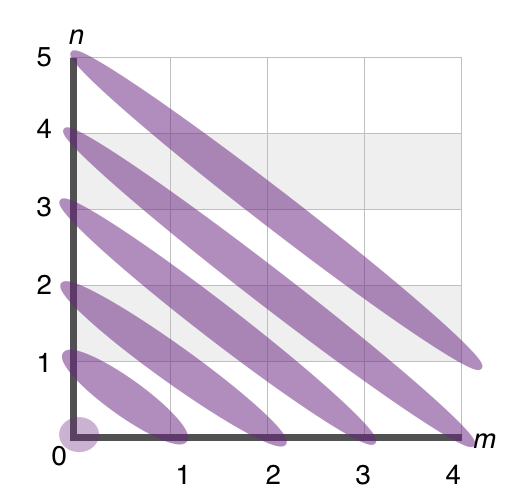
\includegraphics[height=5cm]{diagonal.png}
%\end{center}

 
 \begin{center}
    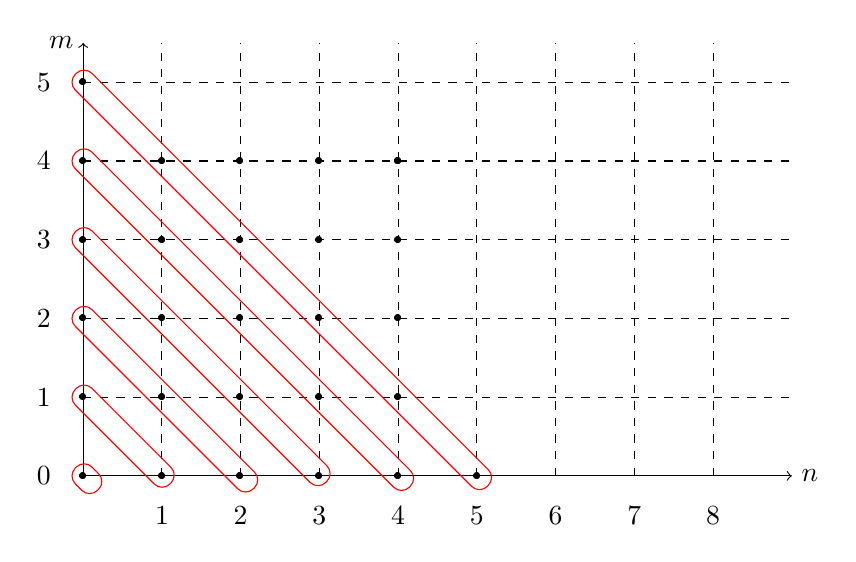
\begin{tikzpicture}
      \draw [->] (0, 0) -- (9, 0) node [right] {$n$};
      \draw [->] (0, 0) -- (0, 5.5) node [left] {$m$};
      \foreach \x in {1,...,8}{
      \draw [dashed] (\x, 0) -- (\x, 5.5);
      \node at (\x,-0.5) {$\x$}; }
      \foreach \y in {1,...,5}{
      \draw [dashed] (0, \y) -- (9, \y);
       \node at (-0.5,\y) {$\y$}; }
    \foreach \Point in {(0,0), (0,1), (1,0), (1,1), (1,2), (1,3), (1,4), (0,2),(0,3), (0,4), (2,0), (2,1), (2,2), (2,3), (2,4), (3,0), (3,1), (3,2), (3,3), (3,4), (4,0),(4,1),(4,2),(4,3),(4,4),(4,4), (0,5), (5,0)}{
    \node at \Point {\tiny \textbullet};
}
	\node at (-0.5,0) {$0$};
       \draw[rounded corners,red,rotate around={-45:(-0.2,0)}] (-0.2,0) rectangle (0.2,0.3);
       \draw[rounded corners,red,rotate around={-45:(-0.2,1)}] (-0.2,1) rectangle (1.5,1.3);
       \draw[rounded corners,red,rotate around={-45:(-0.2,2)}] (-0.2,2) rectangle (3,2.3);
       \draw[rounded corners,red,rotate around={-45:(-0.2,3)}] (-0.2,3) rectangle (4.3,3.3);
              \draw[rounded corners,red,rotate around={-45:(-0.2,4)}] (-0.2,4) rectangle (5.8,4.3);
       \draw[rounded corners,red,rotate around={-45:(-0.2,5)}] (-0.2,5) rectangle (7.2,5.3);
    \end{tikzpicture}
  \end{center} 
 

Assume it does not matter in which order we add up all the terms i.e. we can add the diagonals $m+n = p$. Indeed counting the terms diagonally, writing $m+n = p$:

\begin{align} \nonumber \exp(x)\exp(y) = \sum_{n=0}^{\infty}\sum_{m=0}^{\infty}\frac{x^n}{n!}\frac{y^m}{m!} &= \sum_{p=0}^{\infty}\sum_{n=0}^{p} \left(\frac{x^ny^{p-n}}{p!} \right) \\\vspace*{5pt} \nonumber
&= \sum_{p=0}^{\infty}\sum_{n=0}^{p}\left(\frac{\comb{p}{n} x^n y^{p-n}}{p!}\right) \\\vspace*{5pt} \nonumber
&= \sum_{p=0}^{\infty} \frac{1}{p!} \sum_{n=0}^{p} \comb{p}{n}  x^n y^{p-n} \\\vspace*{5pt} \nonumber
&= \sum_{p=0}^{\infty} \frac{(x+y)^p}{p!} = \exp(x+y)
\end{align}

\end{proof}

We now have $\cos and \sin$. You will prove on Sheet 2 Question 1 that they are $2\pi$-periodic and all the trigonometric formulae that follow, i.e. $\cos(A+B)$ etc. \textit{Remember them, or be able to derive them in 15 seconds!}

\pagebreak

\subsektion{Other Infinite Series}


There is no infinite series for $\log(x)$, i.e.
\[\log(x) \neq \displaystyle{\sum_{n=0}^{\infty} a_n x^n}\text{ for any }a_n\] (try putting $x=0$, and you would get ``$-\infty = a_0$''). But there one for $\log(1+x)$: 

\[\displaystyle{\log(1+x) = 0 + x - \frac{x^2}{2} + \frac{x^3}{3} - \frac{x^4}{4} + \dots = \sum_{n=0}^{\infty} \frac{(-1)^{n+1}x^n}{n} }\]

\[\displaystyle{\frac{1}{1+x} = 1 - x + x^2 - x^3 + x^4 + \dots = \sum_{n=0}^{\infty} x^n(-1)^n, \; |x| < 1 }\]

This is an example of the geometric series $a + ar + ar^2 + \dots = \frac{a}{1-r}, \; |r|<1$. N.B. We could integrate the series for $\frac{1}{1+x}$ to obtain $\log(1+x) + c = x - \frac{1}{2}x^2 + \frac{1}{3}x^3 - \dots$ assuming integrating term by term is allowed. Letting $x = 0 \implies c = 0$. \\

\subsubsektion{The Binomial Series}
The Geometric series is a special case of the Binomial Series:
\[\displaystyle{(1+x)^{\alpha} = 1 + \alpha x + \frac{\alpha(\alpha -1)}{2}x^2 + \dots + \frac{\alpha(\alpha-1)\dots(\alpha-p)}{(p+1)!}x^{p+1} + \dots \quad (\alpha \in \R) }\]

This series converges provided $|x|<1$. Note, if $\alpha \in \N$, then eventually the coefficients become zero and the power series \emph{terminates} as a polynomial of degree $N$. The series then becomes the binomial theorem: $(1+x)^n = \sum_{k=0}^{n} \comb{n}{k} x^k$\\

Proof by: 
\begin{enumerate}
\item Leave it to M1F
\item Induction
\end{enumerate}

\subsektion{Hyperbolic Functions}\vspace*{5pt}

\begin{definition}
We define 
\[\cosh(x) = \text{ Even part of } (e^x)\]	
\[\sinh(x) = \text{ Odd part of } (e^x)\]	
i.e. 
\[
\begin{aligned}
  \cosh(x) &\equiv \frac{1}{2}(e^x + e^{-x})\\[0.2cm]
  \sinh(x) &\equiv \frac{1}{2}(e^x - e^{-x})
\end{aligned}
\]
\end{definition}


These obviously have the series:
\[\cosh(x) = 1 + \frac{1}{2}x^2 + \frac{1}{4!}x^4 + \dots = \sum_{k=0}^{\infty} \frac{x^{2k}}{(2k)!}\] 
(removing the odd powers from $\exp(x)$), and 
\[\sinh(x) = x + \frac{x^3}{6} + \frac{x^5}{5!} + \dots = \sum_{k=0}^{\infty} \frac{x^{2k+1}}{(2k+1)!}\]



  \begin{center}
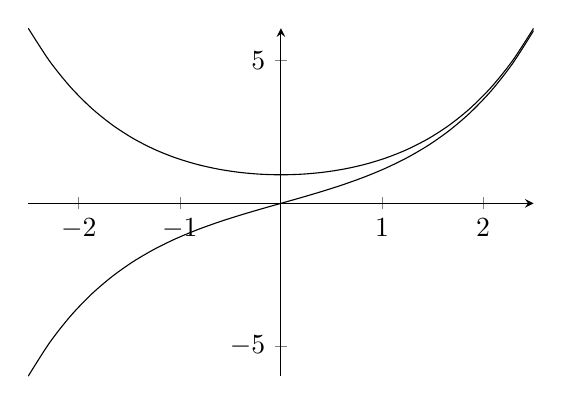
\begin{tikzpicture}
\begin{axis}[
minor tick num=0,
axis y line=middle,
axis x line=middle,
width=8cm,height=6cm
]
\addplot[domain =-2.5: 2.5,smooth] {cosh((x))};
\addplot[domain =-2.5: 2.5,smooth] {sinh((x))};
\end{axis}
\end{tikzpicture}
\end{center}



\subsubsektion{Inverse Hyperbolic Functions}

Suppose 
\[y = \sinh x = \frac{e^{x} - e^{-x}}{2}\]

Solve for $x$. How? Write $u = e^x$:
\[
\begin{aligned}
  2y &= u - \frac{1}{u}\\
  u^2 &- 2uy - 1 = 0\\
  u &= y \pm \sqrt{1 + y^2}
\end{aligned}
\]

\emph{Which root do we take?}

$u e^x > 0\, \forall x$, and $y -\sqrt{1 + y^2} < 0$ (if $y > 0$), so we take the $+$ sign. 
\[e^x = y + \sqrt{1 + y^2}\]
So 
\[
\begin{aligned}
  x &= \log[y + \sqrt{1 + y^2}]\\
  &\equiv \sinh^{-1}y \equiv \mathrm{arcsinh}(y)
\end{aligned}
\]

\emph{What about $\cosh^{-1}$?}

Write 
\[y = \frac{1}{2}(e^x + e^{-x})\]
Letting $u = e^x$ we have 
\[u^2 - 2uy + 1= 0\]
\[\implies u = y \pm \sqrt{y^2-1}\]

\emph{Which root do we take?} Either is possible depending on the domain of $\cosh x$. Assume $x \geq 0 \implies e^x \geq 1$. Again, we need the $+$ sign (for larger root), so 

\[
\begin{aligned}
  x &= \log[y + \sqrt{y^2-1}]\\
  &= \cosh^{-1}y \equiv \mathrm{arccosh}(y)
\end{aligned}
\]

Note: taking the minus sign would give ``$-x$'' instead. Indeed: 
\[\begin{aligned}
  &\log(y + \sqrt{y^2-1}) +\log(y - \sqrt{y^2-1})\\
  &= \log[(y + \sqrt{y^2-1})(y - \sqrt{y^2-1})]\\
  &= \log[y^2 - (\sqrt{y^2-1})^2]\\
  &= \log[y^2 - (y^2 - 1)] = \log(1) = 0
\end{aligned}
\]

So our inverse hyperbolic functions are 
\[
\begin{aligned}
  \sinh^{-1}(x) &= \log(x + \sqrt{x^2 + 1})\\
  \cosh^{-1}(x) &= \log(x + \sqrt{x^2 - 1})
\end{aligned}
\]

Note: $\cosh^2 - \sinh^2 \equiv 1$. There is much similarity with trigonometric functions. 

See Problem Sheet 2 for $\tanh x$ and $\tanh^{-1}x$.  
\[\tanh x \equiv \frac{\sinh x}{\cosh x}\]

  \begin{center}
\begin{tikzpicture}
\begin{axis}[
minor tick num=0,
axis y line=middle,
axis x line=middle,
width=9cm,height=5cm
]
\addplot[domain =-5: 5,smooth] {tanh((x))};
\addplot[dashed] {-1};
\addplot[dashed] {1};
\end{axis}
\end{tikzpicture}
\end{center}

The $\tanh$ function is very useful for switching between $-1$ and $1$ smoothly.
\pagebreak 

\subsektion{Expanding other functions as power series} 

We can use the functions we've defined to express many others as power series.\\
\begin{example}
Find the Power Series expansion for $(1+x^2)\cosh x$
\[
\begin{aligned}
  &(1+x^2)\cosh x\\
  &= (1+x^2)\left(1 + \frac{x^2}{2} + \frac{x^4}{24} + \frac{x^6}{6!} + \dots \right)\\
  &= 1 + \frac{x^2}{2} + \frac{x^4}{24} + \mathcal{O}(x^6)\\
  &+ \quad x^2 + \frac{x^4}{2} + \mathcal{O}(x^6)\\
  &= 1 + \frac{3x^2}{2} + \frac{13}{24}x^4 + \mathcal{O}(x^6)
\end{aligned}
\]

Note: $\mathcal{O}(x^6)$ means terms at least as small as $cx^6$ as $x\to \infty$

\end{example}\vspace*{10pt}

\begin{example}
Find the Power Series expansion for
\[\frac{\sqrt{1 + \frac{x^2}{2}}}{\cos x}\]	

Use the binomial theorem for expanding the numerator: 

\[
\begin{aligned}
  \sqrt{1 + \frac{x^2}{2}} &= \left(1 + \frac{x^2}{2}\right)^{1/2}\\
  &= 1 + \frac{1}{2}\left(\frac{x^2}{2}\right) + \frac{(\frac{1}{2})(-\frac{1}{2})}{2} \left(\frac{x^2}{2}\right)^2 +\frac{(\frac{1}{2})(-\frac{1}{2})(-\frac{3}{2}}{3!} \left(\frac{x^2}{2}\right)^3 + \dots \\
  &= 1 + \frac{x^2}{4} -\frac{x^4}{32} + \mathcal{O}(x^6)
\end{aligned}
\]

Now 
\[\cos x = 1 - \frac{x^2}{2} + \frac{x^4}{4} + \mathcal{O}(x^6)\]

So how do we deal with 
\[\begin{aligned}\frac{1}{\cos x} &= \frac{1}{1 - \frac{x^2}{2} + \frac{x^4}{4} + \mathcal{O}(x^6)}\\
&= \frac{1}{1-T}\end{aligned}\]

Define $T = \frac{x^2}{2} -\frac{x^4}{4!} + \mathcal{O}(x^6)$. 

\[
\begin{aligned}
  \frac{1}{1-T} &= 1 + T + T^2 + \mathcal{O}(T^3)\\
  \frac{1}{\cos x} &= 1 + \left(\frac{x^2}{2} - \frac{x^4}{24}\right) + \left(\frac{x^2}{2} - \frac{x^4}{24}\right)^2 + \mathcal{O}(x^6)\\
  &= 1 + \frac{x^2}{2} - \frac{x^4}{24} + \left(\frac{x^2}{2}\right)^2 + \mathcal{O}(x^6)\\
  &= 1 + \frac{x^2}{2} + \frac{5x^4}{24}
\end{aligned}
\]

Putting them together: 

\[
\begin{aligned}
  \frac{\sqrt{1 + \frac{x^2}{2}}}{\cos x} &= \left(1 = \frac{x^2}{4} - \frac{x^4}{32}\right)\left(1 + \frac{x^2}{2} + \frac{5x^4}{24}\right) + \mathcal{O}(x^6)\\
  &= 1 + x^2\left[ \frac{1}{4} - \frac{1}{2}\right] + x^4\left[1.\frac{5}{24} + \frac{1}{4}\frac{1}{2} - \frac{1}{32}.1\right]\\
  &= 1 + \frac{3x^2}{4} + \frac{x^4}{96}[ 20 + 12 - 3] + \mathcal{O}(x^6)\\
  &= 1 + \frac{3x^2}{4} + \frac{29x^4}{96} + \mathcal{O}(x^6)
\end{aligned}
\]
\end{example}\vspace*{5pt}

\begin{example} A ``simpler'' example: Find the power series for 
\[\frac{1}{1 + e^x}\]

Try letting $T = e^x$: 

\[
\begin{aligned}
  \frac{1}{1 + T} &= 1 - T + T^2 - T^3 + T^4 - T^5 + T^6 - T^7 + \dots\\
  &= -(1 + x + \frac{x^2}{2} + \frac{x^3}{6} + \frac{x^4}{24} + \dots)\\
  &+ (1 + x + \frac{x^2}{2} + \frac{x^3}{6} + \frac{x^4}{24} + \dots)^2\\
  &- (1 + x + \frac{x^2}{2} + \frac{x^3}{6} + \frac{x^4}{24} + \dots)^3\\
  &+ (1 + x + \frac{x^2}{2} + \frac{x^3}{6} + \frac{x^4}{24} + \dots)^4\\
\end{aligned}
\]

We would then try gathering the constant terms, the $x$ terms together etc. But then we end up with $-1 + 1 -1 + 1 - 1 + \dots$ and $x + x + x + \dots$, which goes off to infinity! 

\emph{What's gone wrong?}

 Suppose $x$ is very small, then $T = 1$ which is still large, so there is no justification for neglecting small powers of $T$... we end up having to include all powers of $T$ - for which we are DOOMED. 
 \end{example}

\begin{theorem}[Golden Rule]
	Never ever ever expand in a quantity you are not prepared to treat as small. 
\end{theorem}\vspace*{10pt}


\begin{example}
 We broke the Golden Rule, so start Example 2.4 again: 

Write $T = e^x - 1$.

\[
\begin{aligned}
  \frac{1}{1 +e^x} &= \frac{1}{1 + 1 + T}\\
  &= \frac{1}{2 + T}\\
  &= \frac{1}{2}\left(1 + \frac{T}{2}\right)^{-1}\\
  &= \frac{1}{2}\left( 1 -\frac{T}{2} + \left(\frac{T}{2}\right)^2\right) + \dots \\
  &= \frac{1}{2} - \frac{T}{4} + \frac{T^2}{8} + \dots\\
  &= \frac{1}{2} - \frac{1}{4}\left( x + \frac{x^2}{2} + \mathcal{O}(x^3)\right) + \frac{1}{8}\left(x + \frac{x^2}{2}\right)^2 + \mathcal{O}(x^3)\\
  &= \frac{1}{2} - \frac{1}{4}x - \frac{1}{8}x^3 + \frac{1}{8}x^2 + \mathcal{O}(x^3)\\
  &= \frac{1}{2} -\frac{1}{4}x + \mathcal{O}(x^3)
\end{aligned}
\]
 
 	
\end{example}



 













\subsektion{Maclaurin Series}

\textit{What Kind of functions have a power series?}\lecturemarker{9}{31.10.2014}

i.e. When can we write $\displaystyle{f(x) = a_0 + a_1x + a_2x^2 + \dots a_nx^n = \sum_{n=0}^{\infty} a_nx^n}$?

Note that if this is true then $f(0) = a_0$. So if $f(x)$ is \emph{differentiable} (see later)  and it is legitimate to differentiate an infinite series term by term, then \[f'(x) = a_1 + 2a_2 + \dots na_n = \sum_{n=0}^{\infty} na_nx^{n-1}\] Now we put $x=0$, to get $f'(0) = a_1$.

In general, if the function $f(x)$ can be differentiated $r$ times (and so can the series), then \[f^{(r)}(0) = a_r r!x^0 + 0 + 0 + 0 + \dots \implies \boxed{a_r = \dfrac{f^{(r)}}{r!}}\]

(if $n<r$ in sum, one of the prefactors of $x^{n-r}$ is 0. If $n>r, x^{n-r}$ is 0, when $x=0$. So only one term, $n=r$, remains.)

So formally,\\

\begin{definition} if the function has a power series then we expect the \emph{Maclaurin Series} (or the Taylor series about $x=0$) to be:

\[\displaystyle{f(x) = f(0) + xf'(0) + \frac{x^2f''(0)}{2!} + \dots + \frac{x^rf^{(r)}(0)}{r!} = \sum_{n=0}^{\infty} \frac{f^{(n)}(0)}{n!} x^n}\]

\end{definition}

We suspect therefore, the only those functions with an arbitrary number of derivatives of $x=0$ have the power series expansion.

So $\log(x), x^{3.1}, \sin(x^{\frac{1}{2}}),$ or $|x^3|$ do not have series expansions. There are some functions for which the power series exists but converges to a different function. Such functions are called \emph{non-analytical} functions. e.g.
\[f(x) = \begin{cases}
 e^{-\frac{1}{x^2}} & x \neq 0\\
0 & x=0\\
 \end{cases}\]
 
 We shall not worry about such functions anymore.
 
So a Maclaurin series exists $\iff f^{(n)}(0)$ exists $\forall n$. 

e.g. $f(x) = e^{-x}\sin(2x) = 2x - 2x^2 + \mathcal{O}(x^3)$

\subsektion{Radius of Convergence}\vspace*{5pt}

\begin{definition}
For any power series $\displaystyle{\sum_{n=0}^{\infty} a_nx^n}$ ($a_n, x \in \mathbb{C}$), $\exists \R$ such that:

\begin{itemize}
\item if $|x| < R$ series converges
\item if $|x| > R$ series does not converge
\item if $|x| = R$ anything can happen
\item if $R = 0$ series converges only for $x = 0$
\item if ``$R = \infty$'' series converges $\forall x$
\end{itemize}

$R$ is called the \emph{radius of convergence}
\end{definition}\vspace*{-5pt}


\begin{center}
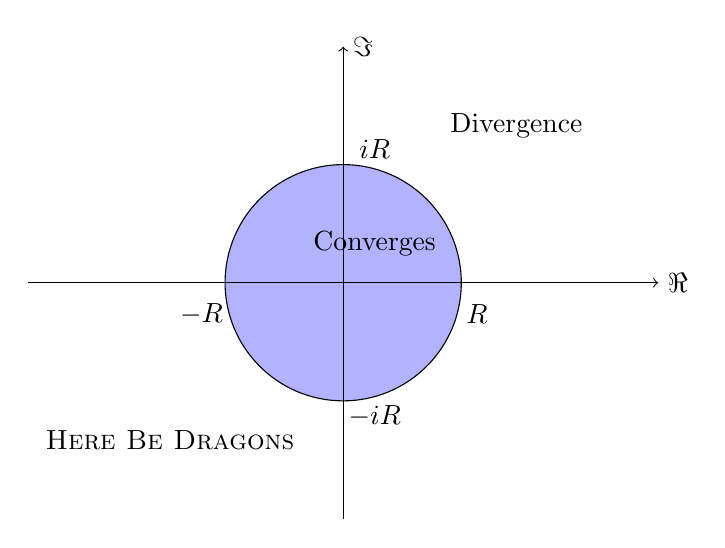
\begin{tikzpicture}
\fill[color =Blue!30] (0,0) circle (1.5);
\draw [->] (-4,0) -- (4,0) node [pos = 1, right] {$\Re$};
\draw [->] (0,-3) -- (0,3) node [pos = 1, right] {$\Im$};
\draw (0,0) circle (1.5);
\node at (0.4,1.7) {$iR$}; 
\node at (0.4,-1.7) {$-iR$}; 
\node at (1.7,-0.4) {$R$}; 
\node at (-1.8,-0.4) {$-R$}; 
\node at (-2.2,-2) {\textsc{Here Be Dragons}};
\node at (2.2,2) {Divergence};
\node at (0.4,0.5) {Converges};
\end{tikzpicture}	
\end{center}


\begin{example}$(x+\alpha)^{\alpha} \quad a \neq 0 \in \R,\, \alpha \in \R$
\[\implies a^{\alpha}(1 + \frac{x}{a})^{\alpha}\]

assuming $a >0$ (otherwise if $a <0$, write $a=-b, (x-b)^{\alpha} = b^{\alpha}(\frac{x}{b} -1)^{\alpha})$
\[= (1+t)^{\alpha}\]
 we ``know'' this requires $|t|<1 \implies |\frac{x}{a}| < 1 \implies |x| < |a|$, so $\boxed{R = |a|}$.
\end{example}\vspace*{5pt}


\emph{What limits the circle of convergence?}

In practice, the series converges in as big a circle as it can i.e. until it reaches a singular point. e.g. $\frac{1}{x^2+1}$ is singular (infinite) when $x=i$, so $R \ngtr 1$ (else series would have to converge at $x = i$, but it can't as function is infinite there), so $R = 1$ for this function.\\


He spent Lecture 10 \lecturemarker{10}{Nov} going through his handout on Analysis. This basically summarises \textsc{M1P1 Analysis I}, the most important results of which are: 

\begin{theorem}[Comparison Test]
Suppose $a_n \geq b_n \geq 0$. Then 
\[\sum_{n=0}^{\infty} a_n \text{ convergent } \implies \sum_{n=0}^{\infty} b_n \text{ convergent }  \]	
\end{theorem}\vspace*{5pt}
 

\begin{theorem}[Ratio Test]
	If $\lim_{n\to \infty} \left|\frac{a_{n+1}}{a_n}\right| = l$, then the series 
	\[\sum_{n=0}^{\infty} a_n \begin{cases}
 \text{ converges if} & l < 1\\
 \text{ diverges if} & l > 1\\
 \text{ uncertain if} & l = 1	
 \end{cases}
\]
\end{theorem}

We can use the ratio test to determine the radius of convergence for a power series, since applying it to $\sum_{n=0}^{\infty} a_n x^n$, we have:  
\[\lim_{n\to \infty} \left|\frac{a_{n+1}x^{n+1}}{a_nx^n}\right| = \frac{|x|}{R}\]

Then by the ratio test, the power series converges if $|x| < R$, diverges if $|x| > R$ and may do either if $|x| = R$. So if the test works, $R$ is in fact the \emph{radius of convergence.}


Recall \lecturemarker{11}{6/11} 
the Maclaurin series: 
\[f(x) = \sum_{n=0}^{\infty} \frac{f^{(n)}(0)x^n}{n!}\]

We can derive the \emph{Taylor series} from the Maclaurin series in a few steps. 

Define a new function 
\[
\begin{aligned}
  g(y + h) &= f(h) \text{ for some constant } y\\
  f'(0) &= g'(y)\\
  f''(g) &= g''(y-h) \text{ etc.} 
\end{aligned}
\]

So we get 
\[g(y+h) = \sum_{n=0}^{\infty} \frac{g^{(n)}(y)h^n}{n!}\]

Relabelling $y \to x$ and $g \to f$, we get the Taylor series:\\

\begin{definition}The \emph{Taylor series} is \[f(x+h) = \sum_{n=0}^{\infty} \frac{f^{(n)}(x)h^x}{n!}\]
\end{definition}\vspace*{5pt}

\begin{center}
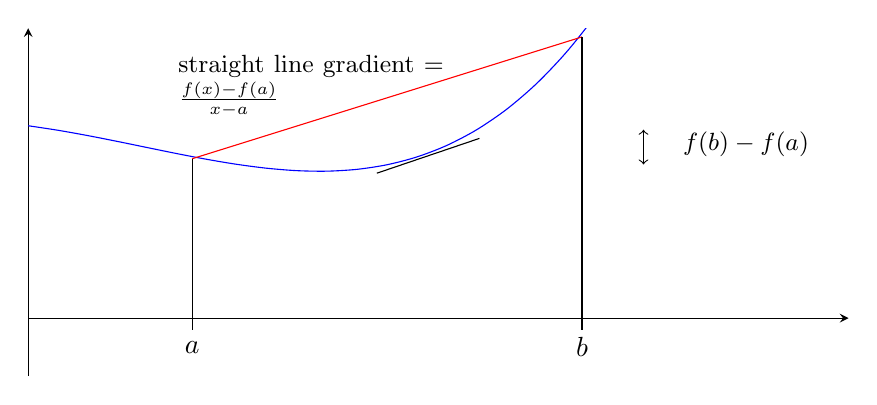
\begin{tikzpicture}
\begin{axis}[
 axis line style={black},
 axis lines=middle,
  ymin = -0.2,
  ymax = 1,
  xmin = 6,
  xmax = 10,
     ytick = 0,
   xtick = 0, 
  width=12cm,height=6cm]
      \addplot[draw=blue, domain=6:9.5,smooth]{0.006*x^4 - 0.0987*x^3 + 0.3937*x^2 + 0.6556*x - 3.9};
       \draw (axis cs:7.7,0.50) -- (axis cs:8.2,0.62); %tangent line
       \draw[red](axis cs:8.7,0.97)--  (axis cs:6.8,0.55); %big tangent line
       \draw (axis cs:8.7,0.97) -- (axis cs:8.7,-0.04) node at (axis cs:8.7,-0.1) {$b$};
       \draw (axis cs:6.8,0.55) -- (axis cs:6.8,-0.04)  node at (axis cs:6.8,-0.1) {$a$};
        \draw[<->] (axis cs:9,0.53) -- (axis cs:9,0.65) node at (axis cs: 9.5,0.6) {\small $f(b) - f(a)$};
         \node[text width=4cm] at (axis cs:7.5,0.8) {\small straight line gradient $= \frac{f(x)-f(a)}{x-a}$};
  \end{axis}
\end{tikzpicture}
\end{center}

What the taylor series does is approximate $b$ by considering the derivatives at $a$.



\pagebreak


\subsubsektion{Finding the Radii of Convergence}\vspace*{5pt}

\begin{example}
\[\exp(x) = \sum_{n=0}^{\infty} \frac{x^n}{n!}\]

To find the radius of convergence, look at the ratio of two adjacent terms. 
\[
\begin{aligned}
  \left|\frac{x^{n+1}/(n+1)!}{x^n/n!}\right|
  &= \frac{|x|n!}{(n+1)!}\\
  &= \frac{|x|}{n+1}
\end{aligned}
\]

Now take the limit as $n \to \infty$. Obviously this tends to $0$. i.e. 
\[\lim_{n\to \infty}\left|\frac{u_{n+1}}{u_n}\right| = 0 < 1\]

So series converges for all $x$ by the ratio test, so ``$R = \infty$''. 
\end{example}\vspace*{5pt}

\begin{example}
Find the radius of convergence for 
\[f(x) = \tan^{-1}(x) = \arctan(x)\]

Differentiating: 
\[
\begin{aligned}
f'(x) &= \frac{1}{1+x^2} \text{ (see later if necessary!)}\\
&= 1 - x^2 + x^4 - x^6 + x^8 + \dots   
\end{aligned}
\]

So assume 
\[f(x) = C + x - \frac{x^3}{3} + \frac{x^5}{5} - \frac{x^7}{7} + \dots + \frac{x^{2n+1}}{2n+1}(-1)^n + \dots\]

When $x = 0$, $\tan^{-1} = 0 \implies C = 0$, so we have the power series for the function: 
\[f(x) = \sum_{n=0}^{\infty} (-1)\frac{x^{2n+1}}{2n+1}\]

To find the radius of convergence, look at 
\[
\begin{aligned}
  &\lim_{n\to \infty}\left|\frac{(-1)^{n+1}x^{2n+3}/(2n+3)}{(-1)^nx^{2n+1}/2n+1}\right|\\
  &= \lim_{n \to \infty} \left|\frac{(-1)x^2(2n+1)}{(2n+3)}\right|\\
  &= |x^2| \lim_{n\to \infty}\left|\frac{2n+1}{2n+3}\right| 
\end{aligned}
\]

\[
\begin{aligned}
    &= |x^2| \lim_{n\to \infty}\left|\frac{1 + \frac{1}{2n}}{1 + \frac{3}{2n}}\right|\\
  &= |x^2| < 1 \iff |x| < 1| \implies R = 1
\end{aligned}
\]


Why is $R = 1$? The function is perfectly well behaved in $\R$: 

\begin{center}
\begin{tikzpicture}
\begin{axis}[
minor tick num=0,
xtick=\empty,
ytick=\empty,
extra y ticks={-90, 90},
extra y tick labels={$-\frac{\pi}{2}$, $\frac{\pi}{2}$},
axis y line=middle,
axis x line=middle,
width=9cm,height=5cm
]
\addplot[domain =-10: 10,smooth] {atan(x)};
\addplot[domain = -10:10, dashed] {-90};
\addplot[domain = -10:10,dashed] {90};
\end{axis}
\end{tikzpicture}
\end{center}

But in the complex plane this function is not nicely behaved - there is a singularity when $x = i$, so $R \not > 1$. 
\end{example}\vspace*{5pt}


\begin{example}Find $R$ for 
\[ \sum_{n=0}^{\infty}\frac{x^2n^2}{2^n(n+1)}\]

Look at 
\[
\begin{aligned}
  &\lim_{n \to \infty} \left|\frac{\frac{x^{n+1}}{2^{n+1}}\frac{(n+1)^2}{(n+2)}}{\frac{x^n n^2}{2^n (n+1)}}\right|\\
  &= \frac{|x|}{2} \lim_{n \to \infty}\left|\frac{(n+1)^2}{n^2(n+2)}\right|\\
  &= \frac{|x|}{2} < 1 \iff |x| < 2
\end{aligned}
\]

So $R = 2$. 
\end{example}\vspace*{5pt}

To find $R$, we need to be able to find limits. This can often be hard. Normally 
\[\lim_{x \to a} f(x) = f(a)\]
if $f$ is continuous, but what if $f(a)$ is hard to evaluate? 

What is ``$\frac{0}{0}$''? It can be anything. Also troublesome is $\frac{\infty}{\infty}$, $0 \times \infty$, $0^{\infty}$, $\infty - \infty$, $1^{\infty}$. 

\emph{How do we cope?}\\

\begin{example} Find
\[\lim_{x \to \infty} x^{1/2}(\sqrt{x+1} - \sqrt{x+4})\]	

Note 
\[
\begin{aligned}
    &\sqrt{x+1} - \sqrt{x+4}\\
    &= (\sqrt{x+1} - \sqrt{x+4})\dfrac{\sqrt{x+1} + \sqrt{x+4}}{\sqrt{x+1} + \sqrt{x+4}}\\
    &= \frac{(x+1) - (x+4)}{\sqrt{x+1} + \sqrt{x+4}}\\
    &= \frac{-3}{\sqrt{x+1}+\sqrt{x+4}}
\end{aligned}
\]

So our limit is now:
\[
\begin{aligned}
  \lim_{x \to \infty} x^{1/2}(\sqrt{x+1} - \sqrt{x+4}) &= \lim_{x \to \infty} \frac{-3x^{1/2}}{\sqrt{x+1}+\sqrt{x+4}}\\
 &= \lim_{x \to \infty} \left[\frac{-3x^{1/2}}{x^{1/2}(1+\frac{1}{x})^{1/2} + x^{1/2}(1 + \frac{4}{x})^{1/2}}\right]\\
 &= \frac{-3}{2} 
\end{aligned}
\]
\end{example}\vspace*{5pt}

\begin{example}
Find 
\[\lim_{x\to 0} \left[(\cosh(\sqrt{x}))^{1/2}\right]\]	
This tends to $1^{\infty}$, which is a problem. But recalling that $\cosh t = 1 + \frac{1}{2}t^2 + \dots$, we can consider the log:
\[\begin{aligned}
log\left[(\cosh(\sqrt{x}))^{1/2}\right] &= \frac{1}{x}\log(\cos\sqrt{x})\\
&\approx \frac{1}{x}\log(1 + \frac{1}{2}(\sqrt{x})^2)\\
&= \frac{1}{x}\log(1 + \frac{1}{2}x)\\
&\approx \frac{1}{x}\left(\frac{1}{2}x\right) = \frac{1}{2}	
\end{aligned}
\]
noting that $\log(1+t) = t - \frac{t^2}{2} + \frac{t^3}{3} + \dots$. 

So
\[\lim_{x \to 0}\left[(\cosh(\sqrt{x}))^{1/2}\right]  = e^{1/2}\]
\end{example}









\sektion{Differentiation}

\subsektion{First Principles Differentiation}

\emph{What is} \lecturemarker{12}{Nov}
\[\lim_{x\to a} (f(x) - f(a))\]
\emph{if $f(x)$ is continuous?} ($=0$ obviously)\\


\emph{What about}
\[\lim_{x \to a} \left[\frac{f(x) - f(a)}{x-a}\right] ?\]

\begin{center}
\begin{tikzpicture}
\begin{axis}[
 axis line style={black},
 axis lines=middle,
  ymin = -0.2,
  ymax = 1,
  xmin = 6,
  xmax = 10,
     ytick = 0,
   xtick = 0,
  width=12cm,height=6cm]
      \addplot[draw=blue, domain=6:9,smooth]{0.006*x^4 - 0.0987*x^3 + 0.3937*x^2 + 0.6556*x - 3.9};
       \draw (axis cs:7.7,0.53) -- (axis cs:8.2,0.65); %tangent line
       \draw (axis cs:8.2,0.65) -- (axis cs:8.2,-0.04) node at (axis cs: 8.2,-0.1) {$x$};
       \draw (axis cs:7.7,0.53) -- (axis cs:7.7,-0.04)  node at (axis cs:7.7,-0.1) {$a$};
        \draw[<->] (axis cs:8.3,0.53) -- (axis cs:8.3,0.65) node at (axis cs: 8.9,0.6) {\small $f(x) - f(a)$};
         \node[text width=4cm] at (axis cs:7.5,0.8) {\small straight line gradient $= \frac{f(x)-f(a)}{x-a}$};
  \end{axis}
\end{tikzpicture}
\end{center}

We are taking the limit of the line joining $(a, f(a))$ to $(x,f(x))$. 
\[\frac{f(x) - f(a)}{x-a} \to \text{ Gradient}\]

\begin{definition}Then as $x \to a$, the limit tends to the gradient of the tangent. If the limit 
\[\lim_{x \to a} \left[\frac{f(x) - f(a)}{x-a}\right] \tag{$*$}\]
exists, we call it the ``\emph{derivative} of the function $f(x)$ at $a$''. 	
\end{definition}

We can denote this limit $(*)$ as either $\dfrac{df}{dx}$ or $f'(x)$. 

If in addition this limit $(*)$ exists for every point on an interval $ c < x < d$ ($x \in (c,d)$), we say $f(x)$ is \emph{differentiable} on the interval $(c,d)$ and we have then defined a new function
\[f'(x) \text{ on } x \in (c,d)\]

\begin{definition}
More commonly we define 
\[f'(x) = \lim_{\epsilon \to 0} \left[\frac{f(x+\epsilon) - f(x)}{\epsilon}\right]\]	
\end{definition}

N.B. This definition is equivalent to $(*)$, with $\epsilon = x-a$. (Exercise: Check this.)

Lets do some examples: 

\begin{example}
Differentiate $f(x) = x^2$ from first principles

\[
\begin{aligned}
  f'(x) &= \lim_{\epsilon \to 0}\left[\frac{(x+\epsilon)^2 - x^2}{\epsilon}\right]\\
  &= \lim_{\epsilon \to 0}\left[\frac{x^2 + 2\epsilon x + \epsilon^2 - x^2}{\epsilon}\right]\\
  &= \lim_{\epsilon \to 0}[2x + \epsilon]\\
  &= 2x
\end{aligned}
\]	
\end{example}\vspace*{5pt}

\begin{example}
Differentiate from first principles $f(x) = x^{1/2}$

\[f'(x) = \lim{\epsilon \to 0}\left[\frac{(x+\epsilon)^{1/2} - x^{1/2}}{\epsilon}\right]\]	

\textbf{Beware} of the temptation to use the binomial series as we haven't proved it!!

We use a trick: $a^2 -b^2 = (a+b)(a-b)$. Let $a = (x + \epsilon)^{1/2}$ and $b = x^{1/2}$, so then:

\[
\begin{aligned}
  f'(x) &= \lim_{\epsilon \to 0}\left[\frac{(x+\epsilon)^{1/2} - x^{1/2}}{\epsilon}\cdot \frac{(x+\epsilon)^{1/2} + x^{1/2}}{(x+\epsilon)^{1/2} + x^{1/2}}\right]\\
  &= \lim_{\epsilon \to 0}\left[\frac{((x+\epsilon)^{1/2})^2 - (x^{1/2})^2}{\epsilon((x+\epsilon)^{1/2} + x^{1/2})}\right]\\
  &= \lim_{\epsilon \to 0} \left[\frac{(x+\epsilon) - x}{\epsilon((x+\epsilon)^{1/2} + x^{1/2})}\right]\\
  &= \lim_{\epsilon \to 0}\left[\frac{\epsilon}{\epsilon((x + \epsilon)^{1/2} + x^{1/2})}\right]\\
  &= \lim_{\epsilon \to 0} \left[\frac{1}{(x + \epsilon)^{1/2} + x^{1/2}}\right]\\
  &= \frac{1}{x^{1/2} + x^{1/2}}\\ 
  &= \frac{1}{2}\frac{1}{x^{1/2}} = \frac{1}{2}x^{-1/2}
\end{aligned}
\]
\end{example}\vspace*{5pt}

\subsubsektion{Product Rule}

Suppose we have $f(x)$ and $g(x)$ that are differentiable, i.e. their derivatives exists. We ask what is the derivative of their product $f(x)\cdot g(x)$??


\[
\begin{aligned}
  \frac{d}{dx}(fg) &= \lim_{\epsilon \to 0}\left[\frac{f(x +\epsilon)g(x+\epsilon)-f(x)g(x)}{\epsilon}\right]\\
  &= \lim_{\epsilon \to 0}\left[\frac{f(x +\epsilon)g(x+\epsilon) +0 -f(x)g(x)}{\epsilon}\right]\\
\end{aligned}
\]


\[
\begin{aligned}
   \frac{d}{dx}(fg) &= \lim_{\epsilon \to 0}\left[\frac{f(x +\epsilon)g(x+\epsilon) - f(x)g(x+\epsilon) + f(x)g(x + \epsilon) -f(x)g(x)}{\epsilon}\right]\\[0.2cm]
  &= \lim_{\epsilon \to 0}\left[g(x+\epsilon)\left(\frac{f(x+\epsilon)-f(x)}{\epsilon}\right) + f(x)\left(\frac{g(x+\epsilon) -g(x)}{\epsilon}\right)\right]\\[0.2cm]
  &= \lim_{\epsilon \to 0}[g(x)+\epsilon]\lim_{\epsilon \to 0}\left(\frac{f(x+\epsilon)-f(x)}{\epsilon}\right) +  \lim_{\epsilon \to 0}[f(x)+\epsilon]\lim_{\epsilon \to 0}\left(\frac{g(x+\epsilon)-g(x)}{\epsilon}\right) \\[0.2cm]
  &= g(x)f'(x) + f(x)g'(x)
\end{aligned}
\]

We have shown:
\[\boxed{(fg)' = f'g + g'f}\]


\subsubsektion{Chain Rule}

Suppose again that $f,g$ are differentiable in appropriate domains, then what is
\[\frac{d}{dx}(f(g(x)))?\]

By definition
\[\frac{d}{dx}(f(g)) = \lim_{\epsilon \to 0} \left[\frac{f(g(x+\epsilon)) - f(g(x))}{\epsilon}\right]\]

\emph{Trick:} We are going to multiply by $1$ in a clever way by multiplying the top and bottom by $g(x+\epsilon) - g(x)$. [We know the answer will have $g'$ in it, but we are not cheating... not really] 

\[
\begin{aligned}
  \frac{d}{dx}(f(g)) &= \lim_{\epsilon \to 0}\left[\frac{f(g(x+\epsilon) - f(g(x))}{\epsilon}\cdot \frac{g(x+\epsilon)-g(x)}{g(x+\epsilon -g(x)}\right]\\[0.2cm]
  &= \lim_{\epsilon \to 0} \left[\frac{f(g(x+\epsilon))-f(g(x))}{g(x+\epsilon)-g(x)}\right]\lim_{\epsilon \to 0}\left[\frac{g(x+\epsilon)-g(x)}{\epsilon}\right]
\end{aligned}
\]\vspace*{10pt}

\emph{Trick}: Let 
\[
\begin{aligned}
  \theta &= g(x+ \epsilon) -g(x)\\
  \implies &g(x+\epsilon) = g(x) + \theta 
\end{aligned}
\]

I claim that $\lim_{\epsilon \to 0}\equiv \lim_{\theta \to 0}$. So
\[\frac{d}{dx}(f(g)) = \lim_{\epsilon \to 0}\left[\frac{g(x+\epsilon)-g(x)}{\epsilon}\right]\;\lim_{\theta \to 0}\left[\frac{f(g(x) + \theta) -f(g(x))}{\theta}\right]\]

Let $g(x) = u$, so 
\[\lim_{\theta \to 0} \left[\frac{f(u + \theta) - f(u)}{\theta}\right] = \frac{df}{du}\]

Then we have 
\[\boxed{\frac{d}{dx}(f(g)) = \frac{dg}{dx}\cdot \frac{df}{du}}\]


\subsubsektion{Quotient Rule} 

\emph{What is} $\dfrac{d}{dx}\left(\dfrac{f(x)}{g(x)}\right)$? 

We will use the product rule: 

\[\left(\frac{f}{g}\right)' = f'\left(\frac{1}{g}\right) + f\left(\frac{1}{g}\right)'\]

\emph{Aside: What is $\left(\frac{1}{x}\right)'$?}

\[
\begin{aligned}
  \lim_{h \to 0}\left[\frac{\frac{1}{x+h} - \frac{1}{x}}{h}\right] &= \lim_{h \to 0}\left[\frac{x - (x+h)}{h(x+h)(x)}\right]\\
  &= \lim_{h \to 0}\left[\frac{-1}{(x+h)(x)}\right]\\
  &= -\frac{1}{x^2} = -x^{-2}. 
\end{aligned}
\]

Therefore 
\[
\begin{aligned}
  \frac{d}{dx}\left(\frac{1}{g}\right) &= \frac{d}{dg}\left(\frac{1}{g}\right)\frac{dg}{dx} \quad \text{[Chain Rule]}\\
  &= -\frac{1}{g^2}\cdot g'
\end{aligned}
\]

Putting it all together, we find: 

\[
\begin{aligned}
  \left(\frac{f}{g}\right)' &= \frac{f'}{g} - \frac{fg'}{g^2}\\
  &= \frac{f'g - fg'}{g^2} 
\end{aligned}
\]

So 
\[\boxed{\frac{d}{dx}\left(\frac{f(x)}{g(x)}\right) = \frac{\frac{df}{dx}g - f\frac{dg}{dx}}{g^2}}\]

With all these rules we can find the derivative to say: $\log(1 + \sin(2^x + \sin(x)^{\cos(x)}))$.\\

















The product rule and chain rule extend to more than two functions e.g. \lecturemarker{13}{10.11.2014}
\[(fgh)' = f'(gh) + f(gh)' = f'(gh) + fg'h + (fg)h'\]

Similarly (by defining $g(h(x)) \equiv k(x)$):\\
 \[f[g(h[x])]' = f[k(x)]' = f'(k(x)).k'(x) = f'(g(h(x)))g'(h(x))h'(x)\]
 
 It's easier to just remember that:
 \[\displaystyle{
 \frac{dy}{dx} = 
 \frac{dy}{du}
 \frac{du}{dt}
 \frac{dt}{d\Omega}
 \frac{d\Omega}{d\chi}
 \frac{d\chi}{d\xi}
 \frac{d\xi}{dx}   
 } \text{ etc. }\]
 
\subsubsektion{Some more ``First Principles'' Differentiation}\vspace*{5pt}

\begin{example}
What is $\dfrac{\mathrm{d}}{\mathrm{d}x} (e^x)$?
\[
\begin{aligned}
&= 
\lim_{\epsilon \to 0} 
\left(\dfrac{e^{x + \epsilon} - e^x}{\epsilon}\right) 
= e^x \lim_{\epsilon \to 0}
\left(\frac{e^x - 1}{\epsilon}\right) 
= e^x \lim_{\epsilon \to 0} 
\left(\frac{1 + \epsilon + \mathcal{O}(\epsilon ^2) -1}{\epsilon} \right) \\
&= e^x \lim_{\epsilon \to 0} 
[1 + \mathcal{O}(\epsilon)]\\
& = e^x
\end{aligned}
\]
\end{example}

\emph{Excerise}: Show that $\dfrac{dx}{dx} = 1$ from first principles

So $1 = \dfrac{dx}{dx} = \dfrac{dx}{dy}\dfrac{dy}{dx}$ (using chain rule). i.e. $\boxed{\dfrac{dy}{dx} = \dfrac{1}{dx/dy}}$


N.B. Next term you will meet partial derivatives, $\frac{\partial u}{\partial x}$; The chain rule for partial differentiation is more complicated, and $\frac{\partial u}{\partial x} \neq \frac{1}{\partial x / \partial u}$ necessarily.\\


\textit{If $y = \log x$, What is $\dfrac{dy}{dx}$?}

Write $x = e^y \implies \dfrac{dx}{dy} = e^y \implies \dfrac{dy}{dx} = \dfrac{1}{e^y} = \dfrac{1}{x}$\\

\subsubsektion{Inverse Trigonmetric Derivatives}

\textit{What is $\dfrac{\mathrm{d}}{\mathrm{d}x} (\sin^{-1} x)$?}

\[
\begin{aligned}
  \dfrac{dx}{dy} &= \dfrac{d}{dy}(\sin y) \\
&= \dfrac{d}{dy}
\left[y - \dfrac{y^3}{6} + \dfrac{y^5}{120} + \dots \dfrac{y^n}{n!}\right] \\
&= \left[1 - \dfrac{y^2}{2} + \dfrac{y^4}{24} + \dots\right]\\
&= \cos y
\end{aligned}
\]

Or we could use first principles:
\begin{align*} \nonumber \frac{d}{dy}[\sin y] 
&= \lim_{\epsilon \to 0}
\left[\frac{\sin(y+\epsilon) - \sin(y)}{\epsilon} \right]\\
&=\lim_{\epsilon \to 0}
 \left[\frac{\sin y \cos \epsilon + \sin \epsilon \cos y - \sin y}{\epsilon} \right] 
 \\ \nonumber
&= \lim_{\epsilon \to 0}
\left[\frac{\sin \epsilon}{\epsilon}\cos y\right]
+ \lim_{\epsilon \to 0}
\left[\sin y \left(\frac{\cos \epsilon -1}{\epsilon} \right) \right]
\\ \nonumber
&=\lim_{\epsilon \to 0}
\left[\frac{\epsilon + \mathcal{O}(\epsilon^3}{\epsilon} \right]\cos y
+ \sin y \lim_{\epsilon \to 0}
\left[\frac{1-\frac{\epsilon^2}{2} + \mathcal{O}(\epsilon^4) -1}{\epsilon}\right]
\\ \nonumber
&= \cos y
\end{align*}


Similarly $\dfrac{d}{dx}(\cos x) = -\sin x$. 

For $\tan(x)$, we have:

\[\begin{aligned}\dfrac{d}{dx}(\tan x) = \left(\frac{\sin(x)}{\cos(x)}\right)
&= 1 + \frac{\sin^2x}{\cot x}\\
&= \frac{\cos^2x + \sin^2x}{\cos^2x}\\
&= \frac{1}{\cos^2x}\\
&= \sec^2x
\end{aligned}\]

Return to $\dfrac{d}{dx}(\sin^{-1}x); \quad x = \sin y$

\[\dfrac{dx}{dy} = \cos y = \sqrt{1 - \sin^2y} = \sqrt{1 - x^2}\]

Hence \[\boxed{\dfrac{dy}{dx} = \dfrac{1}{\sqrt{1-x^2}} = \dfrac{d}{dx}[\sin^{-1}x]}\]

\emph{Exercise}: Show $\dfrac{d}{dx}(\cos x) = -\dfrac{1}{\sqrt{1-x^2}}$\\

Hence $\dfrac{d}{dx}[\sin^{-1}x + \cos^{-1}x] = 0$, which is clear from the right angled triangle: \begin{center}
	
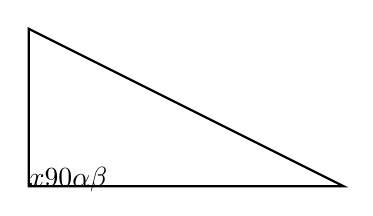
\begin{tikzpicture}[thick]
\coordinate (O) at (0,0);
\coordinate (A) at (4,0);
\coordinate (B) at (0,2);
\draw (O)--(A)--(B)--cycle;

\tkzLabelSegment[below=2pt](O,A){}%{\textit{adjacent leg}}
\tkzLabelSegment[left=2pt](O,B){\textit{$x$}}
\tkzLabelSegment[above right=2pt](A,B){\textit{1}}

\tkzMarkRightAngle[fill=Blue!50,size=0.6,opacity=.4](A,O,B)% square angle here
\tkzLabelAngle[pos = 0.35](A,O,B){~$90\degree$}

\tkzMarkAngle[fill= Blue!50,size=0.8cm,%
opacity=.4](B,A,O)
\tkzLabelAngle[pos = 0.6](B,A,O){$\alpha$}

\tkzMarkAngle[fill= Blue!50,size=0.7cm,%
opacity=.4](O,B,A)
\tkzLabelAngle[pos = 0.5](O,B,A){$\beta$}

\end{tikzpicture}
\end{center}
Since $\alpha = \sin^{-1}x$ and $\beta = \cos^{-1}x$, $\alpha + \beta = \frac{\pi}{2}$, obviously $\frac{d}{dx} \frac{\pi}{2} = 0$.\\



\subsubsektion{Logarithmic Derivative}

\[\displaystyle{
\frac{d}{dx}(\log(u(x))) = \frac{d}{du}\log u.\frac{du}{dx} = \frac{1}{u}u'
}\]

This is called a logarithmic derivative. Useful when performing integration e.g.

\[\displaystyle{
I = \int \frac{e^x + \cos x}{1 + e^x + \sin x} \, \mathrm{d}x
}\]

Observe that $u = 1 + e^x + \sin x$ and $u' = e^x + \cos x$
\[\implies I = \log(1 + e^x + \sin x) + c\]

\subsubsektion{Implicit Differentiation}

If $y$ is given implicitly in terms of $x$ e.g. $y + \tan y = x$, we can differentiate the entire equation term by term with respect to $x$:\\

\begin{example}
Differentiate $y + \tan y = x$:
\begin{align*}\nonumber
\frac{d}{dx}(y + \tan y) = \dfrac{d}{dx}(x) &= 1
\\ \nonumber 
\implies \frac{dy}{dx}\frac{d}{dy}(y + \tan y) &= 1
\\ \nonumber
\implies \frac{dy}{dx}(1 + \sec^2y) &= 1
\end{align*}
\begin{align*}
\implies \frac{dy}{dx} &= \frac{1}{\sec^2y + 1}\\
& = \frac{1}{2 + \tan^2y}\\
& = \frac{1}{2 + (x-y)^2}
\end{align*}
\end{example}



\subsubsektion{Higher Derivatives}

If $f(x)$ is differentiable in $(a,b) \iff f'(x)$ is defined on $(a,b)$.\\

 Maybe $f'$ is also differentiable. If so, we write it as 
 \[f''\text{ or }\dfrac{d^2f}{dx^2}\text{ or }\left(\dfrac{d}{dx}\right)^2f\]
 BUT NOT EVER EVER $\left(\dfrac{df}{dx}\right)^2$
 
 Continuing, we can write the n'th derivative (if it exists) as 
 \[f^{(n)}(x)\text{ or  }\dfrac{d^nf}{dx^n}\text{ or }\left(\dfrac{d}{dx}\right)^n f\]
 These forms are useful for Taylor / Maclaurin series.

\subsektion{Leibniz' Rule}

\textit{How can we (easily) differentiate a product many times?} \lecturemarker{14}{Nov}\\

Suppose $f$ and $g$ are differentiable an arbitrarily number of times. What is $(fg)'$? Use the product rule:

\[
\begin{aligned}
  (fg)' &= f'g + fg'\\
(fg)'' &= (f'g + fg')' = (f'g)' + (fg')' = f''g + 2f'g' + fg''\\
(fg)''' &= f'''g + 3f''g' + 3f'g'' + fg'''
\end{aligned}
\]

We spot a pattern, and make an inspired (but intelligent) guess:


\[
(fg)^n = \left.\sum_{r=0}^n {n \choose k} f^{(r)}g^{(n-r)}
 \quad \right\} \text{ Leibniz' Formula } \quad (*)\]

This is very similar to the binomial theorem:\\
\[\displaystyle{
(f+g)^n = \sum_{r=0}^n {n \choose k} f^{r}g^{n-r}
}\] 
(which I had hoped would have been proved in M1F)

\begin{proof}
Use induction to prove $(*)$\\

(A) Take $n = 1: (fg)' = f'g + fg'$ by product rule, so true for $n=1$

(B) Assume $(*)$ holds when $n=k$, and try to prove it then holds for $n = k + 1$. Hence:

\[
\begin{aligned}
 (fg)^{(k)} &= \displaystyle{\sum_{r=0}^{k}{k \choose r}f^{(r)}g^{(k-r)} }\text{, and differentiate again:}\\
\implies (fg)^{(k+1)} &= \displaystyle{\sum_{r=0}^{k}{k \choose r} \left[f^{(r+1)}g^{(k-r)} + f^{(r)}g^{(k-r+1)} \right] }\\
& = \displaystyle{
f^{(s)}g^{(k+1-s)}\left[{k \choose s-1} + {k \choose s}\right]
}
\end{aligned}
\]\vspace*{5pt}

\begin{lemma}: $\displaystyle{ {k \choose s-1} + {k \choose s} = {k+1 \choose s} }$	
\end{lemma}

\textit{Proof}
\begin{itemize}
\item[A)] Pester Alessio
\item[B)] Pester Emma
\item[C)] Use Pascal's Triangle
\item[D)] Use Factorials
\end{itemize}

Assuming lemma, we obtain: \[(fg)^{(k+1)} = \displaystyle{\sum_{s=0}^{k+1}{k+1 \choose s}f^{(s)}g^{(k+1-s)} }\]as required. 

(C) Hence by induction $(*)$ holds for all natural $\N$.
\end{proof}

Note: Leibniz is very useful is one of the functions $\omega \log$ $f$ is a polynomial, as then the high derivatives vanish (are zero)\\

\begin{example} What is $\dfrac{d}{dx}(x^2\sin x)$?\\

Using Leibniz, $f = \sin x, g = x^2$:

\begin{flalign} \nonumber 
\dfrac{dy}{dx} &= (\sin x)^{(100)}x^2 + {100 \choose 1}\sin x^{(99)}.2x + {100 \choose 2}\sin x^{(98)}.2 + 0 + 0 + \dots 
\\ \nonumber
&= \sin x[x^2 -9900] - 200x\cos x
\end{flalign}
\end{example}\vspace*{5pt}

\begin{example}: What is the Maclaurin series for $y = \sin^{-1}x$?\\

\[
\begin{aligned}
 y' &= \dfrac{1}{\sqrt{1-x^2}},\quad  y'' = x(1-x^2)^{-3/2}\\
&\implies (1-x^2)y'' = xy'
\end{aligned}
\]

Differentiate entire equation $n$ times using Leibniz rule:
\[\displaystyle{
[(1-x^2)y'']^{(n)} = [xy']^{(n)} = xy^{(n+1)} + ny^{(n)}
}\]

Note that:
\[\displaystyle{
[(1-x^2)y'']^{(n)} = (1-x^2)y^{(n+2)} + n(2x)y^{(n+1)} + \frac{n(n-1)}{2}(-2)y^{(n)}
}\]

Hence \[(1-x^2)y^{(n+2)} - (2n+1)xy^{(n+1)} - n^2y^{(n)} = 0\]

So at $x = 0$, we have:
\[y^{(n+1)}(0) = n^2y^{(n)}(0) \quad \forall n\]

Now $y = \sin^{-1}x \implies y(0) = 0$, and $y' = \dfrac{1}{\sqrt{1-x^2}} \implies y'(0) = 1$. This means all even derivatives are zero. Considering the odd derivatives:

\[y^{(3)}(0) = 1, y^{(5)}(0) = 3^2, y^{(7)}(0) = 5^2.3^2\]

So \[\displaystyle{
\sin^{-1}x = \sum_{n =0}^{\infty} \frac{x^{2n+1}}{(2n+1)!}(n-2)^2(n-4)^2 \dots 5^2 \times 3^2 \times 1 
}\]

\end{example}

\pagebreak


\subsektion{Four Theorems and an Example}

\begin{theorem}\lecturemarker{15}{Nov}
Suppose  $f(x)$ is continuous on $[a,b]$ i.e. $a \leq x \leq b$ and differentiable on $(a,b)$ i.e. $a < x < b$. Then $f(x)$ attains its maximum and minimum values somewhere in $[a,b]$. i.e. 
\[\exists c \; a\leq c \leq b, \text{ s.t. } f(c) \geq f(x)\; \forall x \in [a,b]\]

Furthermore, either $c = a$ or $c = b$ or $f'(c) = 0$. 
\end{theorem}


\begin{theorem}[Rolle's Theorem]
	If $f(a) = f(b) = 0$, and $f$ is continuous on $[a,b]$ and differentiable on $(a,b)$, then $\exists$ a point s.t. $f'(c) = 0$, where $a < c < b$. 
\end{theorem}

\begin{proof}[Sketch Proof]

Choose $c$ to be the maximum of $f$ over $[a,b]$. 

Consider 
\[\frac{f(c + \epsilon) - f(c)}{\epsilon} \leq 0 \text{ where } \epsilon > 0\]
because $f(c)$ is a maximum. 

Consider 
\[\frac{f(c) - f(c-\epsilon)}{\epsilon} \geq 0\]

Then take the limit as $\epsilon \to 0$, both tend to $f'(c)$ but one is $\geq 0$, and the other is $\leq 0$. See \textsc{M1P1 - Analysis I}. 
\end{proof}\vspace*{5pt}


\begin{theorem}[Mean Value Theorem]
Suppose $f$ is continuous in $[a,b]$ and differentiable in $(a,b)$. Then $\exists \zeta \in (a,b)$ such that 
\[\frac{f(b) - f(a)}{b-a} = f'(\zeta)\]
\end{theorem}


\begin{center}
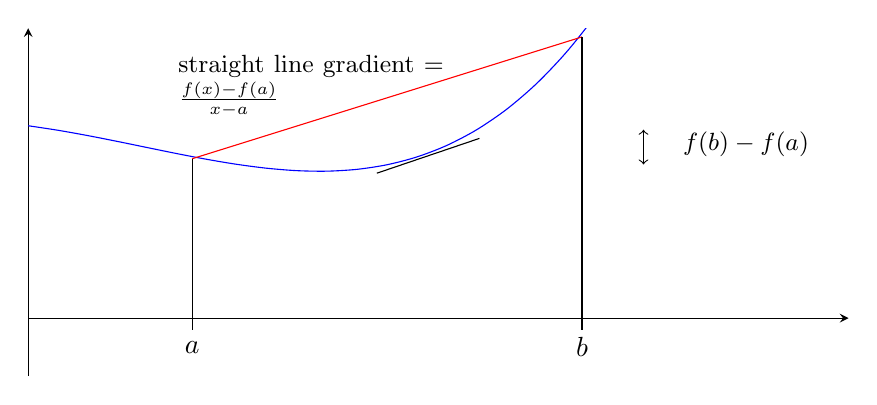
\begin{tikzpicture}
\begin{axis}[
 axis line style={black},
 axis lines=middle,
  ymin = -0.2,
  ymax = 1,
  xmin = 6,
  xmax = 10,
     ytick = 0,
   xtick = 0, 
  width=12cm,height=6cm]
      \addplot[draw=blue, domain=6:9.5,smooth]{0.006*x^4 - 0.0987*x^3 + 0.3937*x^2 + 0.6556*x - 3.9};
       \draw (axis cs:7.7,0.50) -- (axis cs:8.2,0.62); %tangent line
       \draw[red](axis cs:8.7,0.97)--  (axis cs:6.8,0.55); %big tangent line
       \draw (axis cs:8.7,0.97) -- (axis cs:8.7,-0.04) node at (axis cs:8.7,-0.1) {$b$};
       \draw (axis cs:6.8,0.55) -- (axis cs:6.8,-0.04)  node at (axis cs:6.8,-0.1) {$a$};
        \draw[<->] (axis cs:9,0.53) -- (axis cs:9,0.65) node at (axis cs: 9.5,0.6) {\small $f(b) - f(a)$};
         \node[text width=4cm] at (axis cs:7.5,0.8) {\small straight line gradient $= \frac{f(x)-f(a)}{x-a}$};
  \end{axis}
\end{tikzpicture}
\end{center}


Proof in two ways (assuming Rolle's Theorem)

\begin{enumerate}
  \item Proof by Origami
  \item If you are unconvinced, proof by Maths. 
\end{enumerate}

\begin{proof}
Define a new function 
\[g(x) = f(x) - f(a) - \left[\frac{f(b) -f(a)}{b-a}\right](x-a)\]

If $g(a) = g(b) = 0$ and $g$ is continuous and differentiable. 

Now use Rolle's Theorem on $g(x) \implies \exists \zeta \text{ s.t. } g'(\zeta) = 0 \text{ and } a < \zeta < b$. Now $g'(x) = f'(x) - \frac{f(b) = f(a)}{b-a}$, so 
\[0 = g'(\zeta) = f'(\zeta) - \frac{f(b) - f(a)}{b-a}\]

Or
\[f'(\zeta) = \frac{f(b) - f(a)}{b-a}\]
for \emph{some} $\zeta \in (a,b)$.
\end{proof}


\subsektion{De L'Hopital's Rule}\vspace*{5pt}

\begin{theorem}[De L'Hopital's Rule]
If $f(x)$ and $g(x)$ are differentiable in some interval about $x=a$, and $f(a) = g(a)$, and $g'(a) \neq 0$ then 
\[\lim_{x \to a}\frac{f(x)}{g(x)} = \frac{f'(a)}{g'(a)}\]	
or
\[\lim_{x \to a}\frac{f(x)}{g(x)} = \lim_{x \to a}\frac{f'(x)}{g'(x)}\]	
Provided both limits exist [Second one used when $g'(a) = 0$]
\end{theorem}\vspace*{5pt}


\begin{proof}
Use MVT. Assume $x > a$. 
\[\frac{f(x) - f(a)}{x-a} = f'(\zeta)\]
for some $\zeta \in (a,x)$. 

Also 
\[\frac{g(x) - g(a)}{x-a} = g'(z)\]
for some $z \in (a,x)$. 

Now $f(a) = g(a) = 0$. So 

\[\frac{f(x)}{g(x)} = \frac{(x-a)f'(\zeta)}{(x-a)g'(z)} = \frac{f'(\zeta)}{g'(z)}\]
Then 
\[\lim_{x \to a} \left[\frac{f(x)}{g(x)}\right] = \lim_{x \to a}\left[\frac{f'(\zeta)}{g'(z)}\right]\]
Where $\zeta, z \in (a,x)$. 
\end{proof}\vspace*{5pt}


\begin{example}
Find 
\[\lim_{x \to 0}\left[\frac{1-\cos x}{x^2}\right]\]
We could also use power series for $\cos(x)$. 

Using de L'Hopital: 
\[
\begin{aligned}
  &= \lim_{x \to 0}\left[\frac{(1-\cos)'}{(x^2)'}\right]\\
  &= \lim_{x \to 0}\left[\frac{\sin x}{2x}\right]\quad \mbox{ (still ``$0/0$'')}\\
  &= \lim_{x \to 0}\left[\frac{\cos x}{2}\right] = \frac{1}{2}
\end{aligned}
\]
\end{example}\vspace*{5pt}

\begin{example}Find 
\[\lim_{x \to \pi/2} \left[\frac{\cos x}{\log(\pi/2x)}\right]\]

Using de L'Hopital:
\[
\begin{aligned}
  \lim_{x \to \pi/2} \left[\frac{\cos x}{\log(\pi/2x)}\right] &= \lim_{x \to \pi/2}\left[\frac{-\sin x}{-1/x}\right]\\
  &= \frac{-\sin\pi/2}{-1/(\pi/2)} \\ 
  &= 0 
\end{aligned}
\]
\end{example}\vspace*{5pt}





\begin{example}\lecturemarker{16}{20/11}
Find 
\[\lim_{x \to 2} \left[\frac{(x-2)\log(x-1)}{\tan^2\pi x}\right]\]

As $x \to 2$, the numerator $\to 0$, denominator $\to 0$. Se we use Del'hop: [Notice you could replace $\tan$ with $\sin$ since $\cos \to 1$ as $n \to 2$.]

\[
\begin{aligned}
  \lim_{x \to 2} \left[\frac{(x-2)\log(x-1)}{\tan^2\pi x}\right] &= \lim_{n \to 2}\left[\frac{\log(x-1) + \frac{x-2}{x-1}}{2\tan\pi x\cdot \sec^2\pi x\cdot \pi}\right] \\
  &= \frac{1}{2\pi\sec^22\pi} \lim_{x \to 2} \left[\frac{\log(x-1) + \frac{(x-1)-1}{x-1}}{\tan \pi x}\right]\\
  &= \frac{1}{2\pi \cdot 1}\lim_{x \to 2} \left[\frac{\frac{1}{x-1} + \frac{1}{(x-1)^2}}{\pi\sec^2\pi x}\right]\\
  &= \frac{1}{2\pi}\left[\frac{1 + 1}{\pi}\right]\\
  &= \frac{1}{\pi^2}
\end{aligned}
\]	
\end{example}


Note: de L'Hopital's rule also works for expressions of the form ``$\frac{\infty}{\infty}$'', but we haven't justified this. If you believe this, then we can prove:
\begin{proposition} 
\[  \lim_{x \to \infty}\left[\frac{x^n}{e^{\alpha x}}\right] \quad (\alpha, n >0)\]
i.e. Exponentials ``beat'' powers. 
\end{proposition}

\begin{proof}Using de L'Hopital's rule: 
\[
\begin{aligned}
  \lim_{x \to \infty}\left[\frac{x^n}{e^{\alpha x}}\right] 
  &= \lim_{x \to \infty} \left[\frac{nx^n}{\alpha e^{\alpha x}}\right]\\
  &= \lim_{x \to \infty}\left[\frac{n(n-1)x^{n-2}}{\alpha^2e^{\alpha x}}\right]\\
  &= 0
\end{aligned}
\]
\end{proof}
\emph{Is this proof OK?}

\begin{proof}[Alternative Proof.]
Consider 
\[
\begin{aligned}
  0 \leq \frac{x^n}{e^{\alpha n}} &= \frac{x^n}{1 + \alpha x + \frac{1}{2}\alpha^2x^2 + \dots + \frac{1}{(n+1)!}\alpha^{n+1}x^{n+1}}\\
  &< \frac{x^n}{\frac{1}{(n+1)!}\alpha^{n+1}x^{n+1}}\\
  &= \frac{A}{x} \to 0 \text{ as } x \to \infty 
\end{aligned}
\]
\end{proof}

It follows (see Problem Sheet 2) that: 
\[\lim_{n \to 0^+} x^{\alpha}(\log x) = 0\]
(where $\alpha > 0$)

\[\boxed{* \text{ Exponentials ``beat'' powers which ``beats'' logs in any struggle. } *}\]~\\


\subsubsektion{Applications of the Mean Value Theorem}

Recall MVT: If $f$ is continuous and differentiable on $[a,b]$, then $\exists \zeta \in (a,b)$ such that
\[\frac{f(b)-f(a)}{b-a} = f'(\zeta)\]

RHS is unknown. But if $f'$ can be bounded in some way, we can estimate things well.\\

\begin{example}
What is $\sin^{-1}(0.7)$? 

Use the MVT. Let $f(x) = \sin^{-1}(x)$, $a = 0.7, b = \frac{\sqrt{2}}{2} = 0.7071$. Then $\sin^{-1}(b) = \frac{\pi}{4}$. 

Also $f'(x) = \frac{1}{\sqrt{1-x^2}}$, so the MVT says: 
\[\frac{\sin^{-1}(\frac{\sqrt{2}}{2}) - \sin^{-1}(0.7)}{\frac{\sqrt{2}}{2} - 0.7} = \frac{1}{\sqrt{1-\zeta^2}}\]
For $0.7<\zeta < 0.7071$.  

Now $\dfrac{1}{\sqrt{1-x^2}}$ is an increasing function. So 
\[\frac{1}{\sqrt{1-(0.7)^2}} 
< \frac{1}{\sqrt{1-\zeta^2}} 
< \frac{1}{\sqrt{1-\frac{1}{\sqrt{2}}^2 }} = \sqrt{2}\]

\[
\begin{aligned}
  \frac{\frac{\pi}{4} - \sin^{-1}(0.7)}{\frac{1}{\sqrt{2}}-0.7} = \frac{1}{\sqrt{1-\zeta^2}} < \sqrt{2} 
\end{aligned}
\]

\[\begin{aligned}\implies \frac{\pi}{4}-\sin^{-1}(0.7) &< \sqrt{2}(\textstyle{\frac{1}{\sqrt{2}}} - 0.7)\\
&= 1 - 0.7\sqrt{2}\\[0.2cm]
\implies \sin^{-1}(0.7) &> \frac{\pi}{4} -1 + 0.7\sqrt{2}\end{aligned}\]
\end{example}\vspace*{5pt}

\begin{example}
What is $\sin(1)$?

Let $f(x) = \sin x, a = 1, b = \frac{\pi}{3}$. Then by the MVT: 

\[\frac{\sin(\pi/3) - \sin(1)}{\pi/3 -1} = \cos \zeta < 1\]
\[\implies -(\frac{\pi}{3}-1) < \frac{\sqrt{3}}{2} - \sin(1) < \frac{\pi}{3} -1\]
\[\implies \frac{\sqrt{3}}{2} - \frac{\pi}{3} + 1 < \sin(1) < \frac{\sqrt{3}}{2} + \frac{\pi}{3} -1\]	
\end{example}
\pagebreak 

\subsektion{Taylor's Theorem}
\emph{Can we generalise the mean value theorem for functions with many derivative?} \lecturemarker{17}{21/11}

We can write
\[f(x) = f(a) + (x-a)f'(a) + \frac{1}{2}(x-a)^2f''(a) +  \dots + \frac{1}{n!}(x-a)^nf^{(n)}(a) + E_n\]
Where $E_n$ is the error after $n+1$ terms of the Taylor series. 

\begin{theorem}[Taylor's Theorem]
	The error term in the Taylor Expansion
	\[E_n = \int_a^x \frac{f^{(n+1)}(t)(x-t)^n}{n!}\,dt = \frac{(x-a)^{n+1}}{(n+1)!}f^{(n+1)}(\zeta)\]
\end{theorem}

\begin{proof}
We do this by induction. Note that when $n=0$ the RHS is 
\[f(a) + \int_a^x f'(t)\,dt = f(a) + \left[f(t)\right]_a^x = f(a) + f(x) - f(a) = f(x)\]
and equals the LHS.

We assume that Taylor's theorem holds when $n =k$. Then integrating by parts, we have:
\[
\begin{aligned}
  f(x) &= f(a) + (x-a)f'(a) + \dots + \frac{1}{k!}(x-a)^kf^{(k)}(a) + \int_a^x \frac{f^{(k+1)}(t)(x-t)^k}{k!}\,dt\\[0.3cm]
  &= f(a) + \dots + \left[\frac{f^{(k+1)}(t)(x-t)^{k+1}}{k!(k+1)(-1)}\right]_a^x +  \int_a^x \frac{f^{(k+2)}(t)(x-t)^{k+1}}{(k+1)!}\,dt\\[0.3cm]
    &= f(a) + \dots + \frac{f^{(k+1)}(a)(x-a)^{k+1}}{k!(k+1)(-1)} + \int_a^x \frac{f^{(k+2)}(t)(x-t)^{k+1}}{(k+1)!}\,dt
\end{aligned}
\]

So the theorem also holds for $n = k+1$. Hence by induction it holds for all $n \iN$. 

Now by the Intermediate Value Theorem, in the interval $[a,x]$, $f^{(n+1)}$ attains a maximum value $M$ and minimum value $m$:
\[m \leq f^{(n+1)}(t) \geq M\]\vspace*{5pt}
\[  \implies \frac{m(x-t)^n}{n!} \leq \frac{f^{(n+1)}(t)(x-t)^n}{n!} \leq \frac{M(x-t)^n}{n!}\]\vspace*{5pt}
\[\implies \int_a^x\frac{m(x-t)^n}{n!} \leq \int_a^x\frac{f^{(n+1)}(t)(x-t)^n}{n!} \leq \int_a^x \frac{M(x-t)^n}{n!}\]\vspace*{5pt}
\[\implies \frac{m(x-a)^{n+1}}{(n+1)!} \leq \int_a^x\frac{f^{(n+1)}(t)(x-t)^n}{n!} \leq \frac{M(x-a)^{n+1}}{(n+1)!}\]

So for $\zeta \in (a,x)$, we also have \[E_n = \frac{(x-a)^{n+1}}{(n+1)!}f^{(n+1)}(\zeta)\qedhere\]
\end{proof}


Note: If $n = 0$, Taylor's theorem becomes the Mean Value Theorem

\[f(x) = f(a) + E_0 = f(a) + \frac{(x-a)}{1!}f'(\zeta)\]

\begin{example}
\emph{What is $\sinh(1)$}?

\[\sinh = x + \frac{x^3}{3!} + E\]

By taylor's theorem:
\[E = \frac{x^5}{5!}(\sinh\zeta)^{(5)} = \frac{x^5}{5!}\cosh \zeta, \quad 0 < \zeta < x\]

When $x = 1$
\[E = \frac{1}{5!}\cos \zeta, \quad 0 < \zeta < x\]

As $\cosh\zeta = \frac{e^x + e^{-x}}{2}$ is an increasing function, so 

\[\cosh\zeta < \frac{e + e^{-1}}{2} < e < 3\]

So 
\[E < \frac{3}{5!} = \frac{3}{120} = \frac{1}{40} = 0.025\]
\end{example}\vspace*{10pt}


\begin{example}
Improve yesterday's approximation of $\sin(1)$. 

Use Taylor series about $x = \frac{\pi}{3} = a$ in formula: 

\[
\begin{aligned}
  \sin(1) &= \sin(\pi/3) + (1-\pi/3)\cos(\pi/3) + \frac{1}{2}(1-\pi/3)^2(-\sin(\pi/3))\\
   &+ \frac{1}{6}(1-\pi/3)^3(-\cos\pi/3) + \frac{1}{4!}(1-\pi/3)^4\sin\zeta
\end{aligned}
\]
where $1 < \zeta < \pi/3$. 

So approximately: 
\[\sin(1) \approx \frac{\sqrt{3}}{2} + \frac{1}{2}(1-\pi/3) + \frac{1}{2}(1-\pi/3)^2(-\frac{\sqrt{3}}{2}) + \frac{1}{6}(1-\pi/3)^3)-\frac{1}{2})\]

Error $< \frac{1}{24}(\frac{1}{20})^4$ since $\frac{\pi}{3} \equiv 1.0472 < 1.05$. 
\end{example}

So we can reliably and methodically approximate any differentiable function near any point by a polynomial and guarantee that our error is as small as we like. 

Note: General power series expansions about $x = a$ take the form
\[f(x) = c_0 + c_1(x-a) + c_2(x-a)^2 + c_3(x-a)^3 + \dots\]

Let $y = x-a$
\[f(y+a) = g(y) = c_0 + c_1y + c-_2y^2 + \dots\]

If you are asked for an expansion about $x=1$, say, 
\[f(x) = c_0 + c_1(x-1) + c_2(x-1)^2 + \mathcal{O}(x-1)^3\]

\emph{Don't write this as} $d_0 + d_1x + d_2x^2 + \mathcal{O}(x-1)^3$


\subsektion{Stationary Points}

Most important \lecturemarker{18}{21/11} practical use of differentiation is in finding maxima and minima of functions. Formally\vspace*{5pt}

\begin{definition}
A \emph{stationary point} of a differentiable function $f(x)$ is a point $(a, f'(a))$ where $f'(a) = 0$. 
\end{definition}

Such a point may be 
\begin{itemize}
  \item Maximum
  \item Minimum
  \item Neither
\end{itemize}

Near such a point, we can expand (if $f$ is suitably differentiable): 
\[f(x) = f(a) + (x-a)f'(a) + \frac{1}{2}(x-a)^2f''(a) + \frac{1}{6}(x-a)^3f'''(a) + \dots \]

So at a stationary point
\[f(x) = f(a) + \frac{1}{2}(x-a)^2f''(a) + \mathcal{O}(x-a)^3\]
Hence if 
\begin{itemize}
  \item $f''(a) > 0$ we have a local minimum.
  \item $f''(a) < 0$ we have a  local maximum.
  \item $f''(a) = 0$ then we have...
  \[f(x) = f(a) + \frac{1}{6}(x-a)^3f'''(a) + \mathcal{O}(x-a)^4\]

\begin{itemize}
  \item If $f'''(a) \neq 0$, then $f(x)$ increases / decreases as we increase / decrease from $x=a$ - this is neither a maximum or minimum. 


\item If $f'(a) = 0 = f''(a) = f'''(a)$, then we have 
\[f(x) = f(a) + \frac{1}{24}f''''(a)(x-a)^4\]
\end{itemize}

Usually if $f'(a) = 0$, we look at the sign of $f''(a)$ and that would be enough. 
\end{itemize}\vspace*{5pt}

Use your intelligence... for instance\\

\begin{example}
Suppose
\[f'(x) = \sin x e^{-[(x^2 + a^2)^{1/2} + \log[\sinh^{-1}(2x^3)]}\]	

Note that $f'(\pi) = 0$. \emph{What is $f''(\pi)$}? 

At a point where $u = 0$, $(uv)' = u'(a)v(a) + 0$, so 
\[f''(\pi) = \cos\pi e^{-[(\pi^2+a^2)^{1/2} + \dots ]} \]

Alternatively look at the sign of $f'(a-\epsilon)$ and $f'(a+\epsilon)$ as $\epsilon >0$. 
\end{example}

We can also use the fact that a differentiable function on a closed interval attains its maximum and minimum values \emph{either} at an end point \emph{or} at a stationary point.\\

\begin{example}
\[
\begin{aligned}
  f(x) &= x + \frac{1}{x}\\
  f'(a) &= 1 - \frac{1}{x^2} = 0 \text{ at } x = \pm 1
\end{aligned}
\]
Looking at the graph... 

\begin{center}
\begin{tikzpicture}
\begin{axis}[
minor tick num=0,
xtick=\empty,
ytick=\empty,
extra x ticks={0,1},
extra x tick labels={$0$,$1$},
axis y line=middle,
axis x line=middle,
width=9cm,height=5cm
]
\addplot[domain =0: 3,smooth] {x + 1/x};
\end{axis}
\end{tikzpicture}
\end{center}

So $x = 1$ \emph{must} be a minimum. 
\end{example}\vspace*{5pt}

\subsubsektion{Points of Inflexion / Inflection}\vspace*{5pt}

\begin{definition}
	A point of \emph{inflexion} is where $f''(x) = 0$. It is \emph{not} necessary for $f'(x)$ to also be zero. 
\end{definition}


\begin{center}
\begin{tikzpicture}
\begin{axis}[
minor tick num=0,
xtick=\empty,
ytick=\empty,
extra x ticks={0,1},
extra x tick labels={$0$,$1$},
axis y line=middle,
axis x line=middle,
width=9cm,height=5cm
]
\addplot[domain =5: 15,smooth] {(x-10)^3 + 2*(x-10)^2 - 10*(x-10) +100};
\end{axis}
\end{tikzpicture}
\end{center}


By Rolle's Theorem $\exists$ a point where $(f')' = 0$ between the zeros of $f'$. 



\begin{center}
\begin{tikzpicture}
\begin{axis}[
minor tick num=0,
xtick=\empty,
ytick=\empty,
extra x ticks={0,1},
extra x tick labels={$0$,$1$},
axis y line=middle,
axis x line=middle,
width=9cm,height=5cm
]
\addplot[domain =-5:5,smooth] {1/(x^2 + 1)};
\end{axis}
\end{tikzpicture}
\end{center}

\subsubsektion{Curve Plotting} 

It's very important to be able to give a schematic sketch of a function, i.e. the graph $y = f(x)$. This is \emph{not} the best way of defining a curve. $y = f(x)$ has only one $y$ value for each $x$ value. 

\begin{center}
\begin{tikzpicture}
\begin{axis}[
minor tick num=0,
xtick=\empty,
ytick=\empty,
extra x ticks={0,1},
extra x tick labels={$0$,$1$},
axis y line=middle,
axis x line=middle,
width=9cm,height=5cm
]
\addplot[domain =-5:5,smooth] {1/(x^2 + 1)};
\end{axis}
\end{tikzpicture}
\end{center}


\subsektion{Parametric Curves}\vspace*{5pt}


\begin{definition}
The parametric definition is of the form
\[\left. x = f(t), y= g(t) \right\} \text{ in } a \leq t \leq b\]

which defines \emph{any} curve for suitable $f,g$ and parameter $t$.
\end{definition}\vspace*{5pt}

\begin{example}
\[\left. x = t-\sin t, y = 1-\cos t\right\} 0 < t\]	

\emph{What is $\dfrac{dy}{dx}$}? 
\[
\begin{aligned}
  \frac{dy}{dx} &= \frac{dy}{dt} \cdot \frac{dt}{dx} = \frac{dy}{dt} / \frac{dx}{dt}\\
  &= \frac{\sin t}{1-\cos t}\\
  &= \frac{2\sin\frac{t}{2}\cos\frac{t}{2}}{2\sin^2\frac{t}{2}}\\
  &= \cot \frac{t}{2}
\end{aligned}
\]

Now $\dfrac{dy}{dx} = \cot\frac{t}{2}$ is infinite at $t = 0$, $0$ at $t = \pi$, infinite at $t = 2\pi$. 

At $t = 0, x = 0, y = 0$. Note that $0 \leq y \leq 2$. 

\begin{tikzpicture}
    \begin{axis}[
    minor tick num=0,
xtick=\empty,
ytick=\empty,
extra x ticks={3.14,6.28},
extra x tick labels={$\pi$,$2\pi$},
axis y line=middle,
axis x line=middle,
width=15cm,height=5cm,
ymax=3,
            ]
    \addplot [domain=0:5*pi,samples=100]({x-sin(deg(x)},{1-cos(deg(x))}); 
    \addplot[domain = 0:15.7, dashed] {2};
    \end{axis}
    \node at (4,3.5) {$x = t -\sin t$};
     \node at (4,3) {$y = 1-\cos t$};
\end{tikzpicture}

This plots the path of a point on the circumference of a wheel as it moves down a road - a \emph{cycloid}. 

\end{example}

There \lecturemarker{19}{25/11} are more than one way of parameterising a curve.\\

\begin{example}[Hyperbola]

$x^2 - y^2 = 1$. 

\end{example}

\pagebreak

\subsektion{Arc length}

If I move along a curve $y = y(x)$, a small distance 
\[(x,y) \to (x+\delta x, y + \delta x)\]

then the distance moved is $\delta s$ where $\delta s^2 = \delta x^2 + \delta y^2$:

\begin{center}
\begin{tikzpicture}
\draw [->] (0,0) -- (6,0) node[pos = 1, below] {$x$}; 
\draw [->] (0,0) -- (0,4) node[pos = 0.9, left] {$y$};	
\draw[color = blue] (0, 0.2) .. controls (1, 2) and (3, 2.2) .. (5.5, 3.8);
\fill (2,2) circle (2 pt);
\fill (3,2.5) circle (2 pt);
\draw [dashed] (2,2) -- (3,2) node [pos = 0.5,below] {$dx$};
\draw [dashed] (3,2) -- (3,2.5) node [pos = 0.5, right] {$dy$};
\draw [thick] (2,2) -- (3,2.5) node [pos = 0.5, above] {$ds$};
\end{tikzpicture}
\end{center}

More formally: 
\[ds^2 = dx^2 + dy^2 \text{ is the limit as } \delta x \to 0\]
or
\[\left(\frac{ds}{dt}\right)^2 = \left(\frac{dx}{dt}\right)^2 + \left(\frac{dy}{dt}\right)^2\]
\[\lim_{\delta t \to 0}\left(\frac{\delta x}{\delta t}\right) = \frac{dx}{dt}\]
by definition. 

\begin{center}
\begin{tikzpicture}
\draw [->] (-0.5,0) -- (9,0) node[pos = 1, below] {$x$}; 
\draw [->] (0,-0.5) -- (0,5.5) node[pos = 0.9, left] {$y$};	
\draw[color = blue] (0, 0.6) .. controls (2, 0.5) and (3, 1.5) .. (7, 5.2);
\fill (2.8,1.5) circle (2 pt);
\draw [dashed] (2.8,1.5) -- (5,1.5) node [pos = 0.5,below] {\small $1/\sqrt{1+y'^2}$};
\draw [dashed] (5,1.5) -- (5,3) node [pos = 0.5, right] {\small $|y'|/\sqrt{1+y'^2}$};

\draw [->] (2.8, 1.5) -- (5,3) node [anchor = south west] {$\hat{v}$};
\draw [->] (2.8, 1.5) -- (1.5, 3.5) node [anchor = south east] {$\hat{n}$};
      
\draw [dashed] (1.5,3.5) -- (1.5, 1.5) node [pos = 0.5, left] {\tiny $1/\sqrt{1+y'^2}$};
\draw [dashed] (1.5,1.5) -- (2.8,1.5) node [pos = -0.1, below] {\tiny $|y'|/\sqrt{1+y'^2}$};

\end{tikzpicture}
\end{center}
\[\tan \psi = \dfrac{dy}{dx}, \cos\psi = \dfrac{dx}{ds}, \sin\psi = \dfrac{dy}{ds}\]

\begin{definition}
\[\begin{rcases*}
s \text{ \emph{arc length}}\\
\psi \text{ \emph{tangent angle}}	
\end{rcases*} \text{ these are known as \emph{intrinsic coordinates}}
\]
\end{definition}


\begin{definition}
As we move along a curve,, the tangent angle, $\psi$ may change. We define the \emph{curvature}, $\kappa$, to be 
\[\kappa = \frac{d\psi}{ds}\]	
The rate of change of angle with distance along the curve. 
\end{definition}

\emph{How can we relate this to Cartesian coordinates}? 

\[\tan\psi = \frac{dy}{dx}, \cos\psi = \frac{dx}{ds}, \kappa = \frac{d\psi}{ds} = \frac{d\psi}{dx}\frac{dx}{ds}\]

Differentiate $\tan\psi$ with respect to $x$ implicitly
\[\implies \frac{d^2y}{dx^2} = \frac{d}{Dx}(\tan\psi) = \sec^2\psi\frac{d\psi}{dx}\]

Hence 
\[\kappa = \frac{\cos\psi\frac{d^2y}{dx^2}}{\sec^2\psi} = \frac{y''}{\sec^2\psi}\]

Now $\sec^2\psi = 1 + \tan^2\psi = 1+\left(\frac{dy}{dx}\right)^2$. Hence 
\[\boxed{\kappa = \frac{y''}{(1 + (y')^2)^{3/2}}}\]
where $y' = \frac{dy}{dx}$, $y'' = \frac{d^2y}{dx^2}$.\\

\begin{definition}
We also define the \emph{radius of curvature}. 
\[\rho = \frac{1}{\kappa} = \frac{ds}{d\psi} = \frac{(1 + (y')^2)^{3/2}}{y''}\]
\end{definition}

This is the radius of the osculating circle: 
\begin{center}
  \begin{tikzpicture}
    %\draw [->] (0, 0) -- (3, 0) node [right] {$\frac{\Delta \vec{r}}{\Delta t}$};
    %\draw [->] (0, 0) -- (2.2, 0.5) node [above] {$\vec{v}(t)$};
    %\draw [->] (-1.5, -1.5) -- (0, 0) node at (0,-0.5) {$\vec{r}(t)$};
    %\draw [->] (-1.5, -1.5) -- (2, 0) node at (2,-0.5) {$\vec{r}(t+\Delta t)$};
    \draw[color = blue] (-1.5, -0.5) .. controls (0, 0.3) and (2, 1) .. (4, -2.5);
    \draw [dashed] (0.7,-1.65) circle [radius = 1.8];
    \draw (0.7,-1.65) -- (0.9,0.15) node [pos = 0.5, left] {$\rho$};
    \draw [->] (0.95,0.1) -- (0.82,-1.2) node [pos = 0.9, right] {$\hat{n}$};
    \draw [->] (0.9,0.15) -- (2,-0.05) node [right] {$\hat{v}$};
    %\node[color = red] at (0.7,-0.15) {$\Delta \vec{r}$};
	%\draw[color = red, ->] (0,0) -- (2,0);
  \end{tikzpicture}
\end{center}




\subsektion{Polar Coordinates}\vspace*{5pt}

 \lecturemarker{20}{21/11}
\begin{definition} Given a point $(x,y)$ we can define 
\[r = \sqrt{x^2 + y^2} \geq 0\]
and 
\[
\begin{aligned}
  \theta = \begin{cases}\arctan(y/x) &\text{ if } x > 0\\
  \pi - \arctan(y/x) &\text{ if } x < 0
  \end{cases}
\end{aligned}
\]
\end{definition}


  \begin{center}
    \begin{tikzpicture}
      \draw [->] (0, 0) -- (4, 0) node [right] {$x$};
      \draw [->] (0, 0) -- (0, 2.5) node [above] {$y$};
      \draw [dashed] (2.5,0) -- (2.5,2) node [pos = 0.5, right] {$y$};
      \node at (1.6,-0.3) {$x$};
      \draw (0, 0) -- (2.5, 2) node [circ]{} node [pos = 0.6, anchor = south east] {$r$};
      \draw (0.7, 0) arc (0:45:0.7);
      \node at (0.9, 0.3) {$\theta$};
    \end{tikzpicture}
  \end{center}
  
Our definition of $\theta$ is cumbersome, ugly, confusing and messy, so we instead define

\[\theta := \begin{cases}
 \cos\theta &= \frac{x}{r}\\
 \sin\theta &= \frac{y}{r}	
 \end{cases} \quad \text{ say } 0 \leq \theta < 2\pi
\]
\[\boxed{\implies x = r\cos\theta, y = r\sin\theta}\]

We can define a curve by $r = f(\theta)$ if we want.\\ 

\begin{example}
\[r = \frac{l}{1 + e\cos\theta}\]	
Where $l$ and $e$ are constants. (See \textsc{M1A1 Mechanics}) 

\emph{How do we plot such a curve}?

\begin{itemize}
  \item[(a)] Join the dots. Find points on the curve to get an idea of how it looks.
  
  \item[(b)] Regard Polar Coordinates as a parametric definition.

	We know
\[\begin{aligned}
	&x = r\cos\theta, y = r\sin\theta, r = \frac{1}{1-2\cos\theta}  \\[0.2cm]
\implies &x = \frac{\cos\theta}{1-2\cos\theta}, y= \frac{\sin\theta}{1-2\cos\theta}
\end{aligned}\] 
	
\item[(c)] Try to transform to Cartesian.
\[
\begin{aligned}
    r = \frac{1}{1-2\cos\theta} &\implies r - 2r\cos\theta = 1\\
    &\implies r = 1 + 2x\\
    &\iff \sqrt{x^2 + y^2} = 1+2x\\
    &\implies x^2 + y^2 = (1+2x)^2 = 4x^2 + 4x + 1\\
    &\implies 3x^2 + 2x - y^2 + 1 = 0
\end{aligned}
\]
Squaring introduces spurious branch of hyperbola. We need to try another approach...

\[
\begin{aligned}
  r = \frac{1}{1 + e\cos\theta} &\implies r + ex = 1\\
  &\implies r^2 = (1-ex)^2\\
  &\implies x^2 + y^2 = 1-2ex + e^2x^2\\
  &\implies x^2(1-e^2) + 2ex + y^2 = 1
\end{aligned}
\]

We have a conic: 
\begin{itemize}
  \item $e = 0$ - Circle
  \item $e = 1$ - Parabola
  \item $0 < e < 1$ - Ellipse
  \item $e > 1$ - Hyperbola
\end{itemize}

\[
\begin{aligned}
  &x^2 + \frac{2e}{1-e^2}x + \frac{y^2}{1-e^2} = \frac{1}{1-e^2}\\
  &\implies \left(x + \frac{e}{1-e^2}\right)^2 +  \frac{y^2}{1-e^2} = \frac{1}{1-e^2}
\end{aligned}
\]
So the foci is at $\left(-\dfrac{e}{1-e^2},0\right)$.   
\end{itemize}
\end{example}\vspace*{5pt}

Sometimes we cannot easily transform to Cartesian. e.g. $r = \frac{1}{\theta}$ for $\theta >0$. 






\sektion{Integration}
\subsektion{The Riemann Integral}

\emph{Note: Covered rigorously in \textsc{M2PM2 Analysis II}.}\\

\begin{definition} \lecturemarker{21}{21/11}
Given an interval $[a,b]$, we define a \emph{partition} to be a set of $n$ points, $x_1,x_2,\dots,x_n$ such that 
\[a \equiv x_0 < x_1 < x_2 < \dots < x_n < x_{n+1} \equiv b\]	
For a given partition, we choose points on each subinterval, $\xi_0, \xi_1,\dots \xi_n$ such that for all $i$, $x_i < \xi_i < x_{i+1}$. Then for each function $f(x)$, we define the \emph{Riemann sum} to be
\[S_n = (x_1 - x_0)f(\xi_0) + (x_2 - x_1)f(\xi_1) + \dots + (x_{n+1}-x_n)f(\xi_n)\]

\end{definition}

Pictorially, we are forming $n+1$ rectangles whose sum resembles the area under the curve $y = f(x)$. The upper sum is the total area of the red rectangles, while the lower sum is the total area of the black rectangles:
\begin{center}
  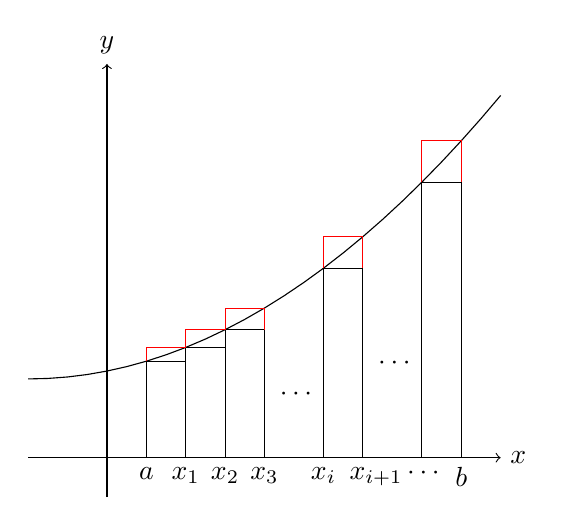
\begin{tikzpicture}
    \draw [->] (-1, 0) -- (5, 0) node [right] {$x$};
    \draw [->] (0, -0.5) -- (0, 5) node [above] {$y$};

    \draw [domain=-1:5] plot (\x, {(\x + 1)*(\x + 1)/10 + 1});

    \draw (0.5, 0) node [below] {$a$} -- (0.5, 1.225) -- (1, 1.225);
    \draw (1, 0) node [below] {$x_1$} -- (1, 1.4) -- (1.5, 1.4);
    \draw (1.5, 0) node [below] {$x_2$} -- (1.5, 1.625) -- (2, 1.625) -- (2, 0) node [below] {$x_3$};
    \node at (2.4, 0.8) {$\cdots$};
    \draw (2.75, 0) node [below] {$x_i$} -- (2.75, 2.40625) -- (3.25, 2.40625) -- (3.25, 0) node [anchor = north west] {$\!\!\!\!\!x_{i + 1}\cdots$};
    \node at (3.65, 1.2) {$\cdots$};
    \draw (4, 0) -- (4, 3.5) -- (4.5, 3.5) -- (4.5, 0) node [below] {$b$};

    \draw [red] (0.5, 1.225) -- (0.5, 1.4) -- (1, 1.4) -- (1, 1.625) -- (1.5, 1.625) -- (1.5, 1.9) -- (2, 1.9) -- (2, 1.625);
    \draw [red] (2.75, 2.40625) -- (2.75, 2.80625) -- (3.25, 2.80625) -- (3.25, 2.40625);
    \draw [red] (4, 3.5) -- (4, 4.025) -- (4.5, 4.025) -- (4.5, 3.5);
  \end{tikzpicture}
\end{center}

We now let $n \to \infty$ in such a manner than $(x_{i+1} - x_i) \to 0$ for all $i$.\\

\begin{definition}If the sequence $S_n$ tends to a limit, and if this limit does not depend on the particular partitions nor the value of $\xi$ we choose, we can write this as the \emph{definite integral} of $f(x)$ between $x=a$ and $x=b$. 
\[\lim_{n \to \infty} S_n = \int_a^b f(x)\, dx\]

The function $f(x)$ is the \emph{integrand}.
\end{definition}
As the integral is a generalisation of a sum, it behaves similarly to one. Various properties follow from the definition, for example: 

\begin{theorem}[Mean Value Theorem for Integrals]
	Suppose $f$ is integrable in $[a,b]$. Then $\exists \xi \in (a,b)$, such that 
	 \[\int_a^b f(x)\,dx = (b-a)f(\xi)\]
\end{theorem}

\begin{proof}
Being integrable, $f$ is bounded by $m \leq f(x) \leq M$, so then 
\[m(b-a) \leq \int_a^b f(x)\,dx \leq M(b-a)\]

Suppose $m$ and $M$ are the minimum and maximum values attained by a continuous function $f$ over $[a,b]$ then $(b-a)f(x)$ attains every value between $(b-a)m$ and $(b-a)M$ in $[a,b]$. In particular the value equal to the integral.
\end{proof}



\begin{theorem}[Fundamental Theorem of Calculus]
Differentiation is the reverse of integration:
	\[\frac{d}{dx}\int_a^x f(t)\, dt = f(x)\]
\end{theorem}
\begin{proof}
If we fix the lower limit $a$ then $f(x)$ defines another function:

\[F(x) = \int_a^x f(t)\,dt\]

It follows that for any $c$ and $d$

\[\int_c^d f(t)\,dt = \int_a^d f(t)\,dt - \int_a^c f(t)\,dt = F(d) - F(c).\]

Consider now 
\[\int_x^{x+h} f(t)\,dt = F(x+h_) - F(x)\]

By the Mean Value Theorem for Integrals (Theorem 4.2), $\exists \xi \in (x,x+h)$ such that
\[F(x+h) - F(x) = (x+h-x)f(\xi)\]

Thus
\[\lim_{h \to 0}\left[\frac{F(x+h) - F(x)}{h}\right] = \lim_{h \to 0}f(\xi)\]

As $h \to 0$, $\xi \to x$. Thus the limit on the RHS exists and equals $f(x)$, and so $F(x)$ is differentiable with derivative $f(x)$, so
\[\frac{d}{dx}\int_a^x f(t)\, dt = f(x)\]
\end{proof}


\emph{What sort of functions are integrable?} 

\begin{itemize}
  \item[(a)] Continuous functions. $f$ continuous on $[a,b] \implies \int_a^b f(x)\, dx$ exists
  \item[(b)] Functions with a single \emph{finite} jump
  \item[(c)] Functions with a finite number of finite jumps
  \item[(d)] If there are an infinite number of discontinuities we're not sure. Integrable.
  \item[(e)] If the function has an infinite discontinuity (i.e. it is unbounded) integral may or may not exist.
  \item[(f)] If either or both limit ($a$ or $b$) is infinite, the integral may or may not exist. 
\end{itemize}

(e) and (f) are important. 

\subsektion{Integrals over infinite ranges}

\emph{Does $\int_0^{\infty} f(x)\,dx$ exist?} 

Assume $f(x)$ is continuous. 

\[\int_0^{\infty} f(x)\,dx = \lim_{N \to \infty} f(x)\,dx\]
Clearly 
\begin{itemize}
  \item[(a)] $f(x) = x$, the limit does not exist $\int_0^N x\,dx = \frac{1}{2}N^2 \to \infty$
  \item[(b)] $f(x) = 1$ limit does not exist similarly.
 \item[(c)] $f(x) = \sin x$ 
\end{itemize}\vspace*{5pt}

We might surmise that a necessary condition for $\int_0^{\infty} f(x)\,dx$ to exist is that $f(x) \to 0$ as $x \to \infty$. In fact this is not true. $\int_0^{\infty} \sin(x^2)\,dx$ does not exist - this is not obvious. 

What is true, is that if $\lim_{x \to \infty} f(x) = A \neq 0$, then integral does not exist. 

Suppose $f(x) \to 0$ as $x \to \infty$. In particular, if $f(x) \approx \frac{1}{x^a}$ as $x \to \infty$, then $\int_0^{\infty} f(x)\, dx$ exists iff $\alpha > 1$.\\

\lecturemarker{22}{21/11} 
\begin{theorem} If $f(x)$ is integrable and $|f(x)| < \frac{A}{x^{\alpha}}$ as $x \to \infty$ if $\alpha > 1$. Then $\int^{\infty} f(x)\, dx$ exists. 
\end{theorem}

\emph{What if $f(x)$ has an infinite discontinuity}?\\

E.g. \[f(x) = \begin{cases}
 \frac{1}{x^2} & \mbox{ if $x \neq 0$}\\
 1 & \mbox{ if $x = 0$}	
 \end{cases}
\]	
\emph{Does $\displaystyle{\int_{-1}^1 f(x)\,dx}$ exist?}

Look at 
\[\int_{-1}^{-\delta} + \int_{-\delta}^{\epsilon} + \int_{\epsilon}^1 \mbox{, where $\delta, \epsilon >0$. 
}\]

So only the behaviour very close to the singularity is important.\\

Consider 
\[\int_0^! \frac{1}{x^{\alpha}}\,dx \text{, define as }\lim_{\epsilon \to 0^+}\int_{\epsilon}^1 \frac{1}{x^{\alpha}}\,dx\]

Then we consider
\[\frac{[x^{1-\alpha}]_{\epsilon}^1}{1-\alpha} = \frac{1-\epsilon^{1-\alpha}}{1-\alpha}\]
Exercise: Calculate $\lim_{\alpha \to 1}$ of the equation. 

Now let $\epsilon \to 0$:
\begin{itemize}
  \item If $\alpha > 0$. $\epsilon^{1-\alpha} \to \infty \implies$ integral does not exist. 
  \item If $\alpha < 1$, $\epsilon^{1-\alpha} \to 0\implies$ integral does exist. 
  \item If $\alpha = 1$, we get $\int_{\epsilon}^1 \frac{1}{x}\,dx = \log \epsilon \to \infty$ as $\epsilon \to 0$. 
\end{itemize}\vspace*{5pt}

So if $f \to \infty$ at $x = 0$ and otherwise continuous, $\int_0^1 f\,dx$ will exist if $f \approx \frac{1}{x^\alpha}$ where $\alpha < 1$ near $x = 0$. Similarly if $f(x)$ has a singularity at $x =c$ say, we need $f \approx \frac{1}{(x-c)^{\alpha}}$ where $\alpha < 1$ near $x=c$ for integral to exist.\\

\begin{example}
\[\int_0^x \frac{e^x}{(x-1)^{1/3}}\
,dx\]	

The only problem is at $x=1$. Near $x=1$, 
\[\text{Integral} \approx \int\frac{e}{(x-1)^{1/3}}\,dx\]
The power is $-\frac{1}{3}$ at the singularity, so as $\alpha = \frac{1}{3} < 1 \implies$ integral does exist.
\end{example}

Functions with a finite number of (``$\alpha < 1$''), ``not too bad'' infinite singularities as integrable.\\

\begin{example}
%What is $\int_0^{\frac{3\pi}{4}} \sec^2x\,dx$?
\[
\begin{aligned}
  \int_0^{\frac{3\pi}{4}} \sec^2x\,dx &= \left[\tan x\right]_0^{\frac{3\pi}{4}}\\
  &= \tan \frac{3\pi}{4} - \tan 0\\
  &= -1
\end{aligned}
\]
But... $\sec^2x > 0 \implies \int \sec^2x> 0$.\\

\emph{So what has gone wrong?} $\sec^2x$ has a singularity at $x = \frac{\pi}{2}$: 


  \begin{center}
\begin{tikzpicture}
\begin{axis}
        [
    ymin=0,ymax=5,
    xmin=0,xmax=3.5,
    %clip=false,
    xtick=\empty,
    extra x ticks={1.5708},
    extra x tick labels={$\frac{\pi}{2}$},
    every extra x tick/.style={
            xticklabel style={anchor=north west},
            grid=major,
            major grid style={dashed,black}
    },
    axis lines = center,
    xlabel=$x$,ylabel=$y$,
    width=8cm,height=5cm
    ]
    \addplot [black, domain = 0:1.50, smooth] {sec(deg(x))^2};
      \addplot [black, domain = 2:3.5,smooth] {sec(deg(x))^2};
\end{axis}
\end{tikzpicture}
\end{center}




\[
\begin{aligned}
  \cos x &\approx \textstyle{\cos\frac{\pi}{2} + (x-\frac{\pi}{2})(-1) + \frac{1}{2}(x-\frac{\pi}{2})^2\cdot 0}\\
  &= 0 + \textstyle{(\frac{\pi}{2} - x)}
\end{aligned}
\]

Near $x = \frac{\pi}{2}$, $\sec^2x = \frac{1}{(\frac{\pi}{2}-x)^2}$. So $\alpha = 2 > 1 \implies$  not integrable. 

Hence 
\[\int_0^{\frac{3\pi}{4}}\sec^2x\,dx = ``\infty" \neq -1\]
\end{example}

\begin{warning} Important to look at Infinities!! \end{warning}


\begin{theorem}[Integration by Substitution]
 \[\int_{\phi(a)}^{\phi(b)} f(x)\,dx = \int_a^b f(\phi(t))\phi'(t)\,dt\]
\end{theorem}
\begin{proof}
Using the chain rule: 
\[
\begin{aligned}
  \frac{d}{dx}\left[F(\phi(t))\right] &= F'(\phi(t))\cdot\phi'(t)\\
  &= f(\phi(t))\cdot\phi'(t)
\end{aligned}
\]

Suppose $F(x) = \int^x f(s)\,ds$, then $F'(x) = f(x)$. Now integrating with respect to $t$: 
\[
\begin{aligned}
  \int_a^b \frac{d}{dt}\left[F(\phi(t))\right]\,dt &= \int_a^b f(\phi(t))\cdot\phi'(t)\,dt\\
  F(\phi(b)) - F(\phi(a)) &= \int_a^b f(\phi(t))\cdot\phi'(t)\,dt\\
  \int_{\phi(a)}^{\phi(b)} f(x)\,dx &+ \int_a^b f(\phi(t))\cdot\phi'(t)\,dt
\end{aligned}
\]
\end{proof}

So starting with 
\[ \int_{\phi(a)}^{\phi(b)} f(x)\,dx\]
we can make a substitution $x = \phi(t)$. Replace $dx$ by $\phi'(t)\,dt$ and replace the limits accordingly. This is very useful for evaluating integrals. But this is even more useful:\\

\begin{theorem}[Integration by Parts]
\[\int_a^b uv'\,dx = [uv]_a^b - \int_a^bu'v\,dx\]
\end{theorem}
\begin{proof}
	Recall the product rule: $\frac{d}{dx}(uv) = \frac{du}{dx}v + \frac{dv}{dx}u$. 
	
	\[
\begin{aligned}
  \int_a^b \frac{d}{dx}(uv)\,dx &= \int_a^b \frac{du}{dx}v\,dx + \int_a^b u\frac{du}{dx}\,dx\\
  [uv]_a^b &= \int_a^b u'v\,dx + \int_a^b uv'dx\\
 \implies \int_a^b uv'\,dx &= [uv]_a^b - \int_a^b u'v\,dx
\end{aligned}
\]
\end{proof}

This enables us to transform an integral into another integral which may be easier to evaluate, for example:\\

\begin{example}\lecturemarker{23}{4/12}
\[\int_0^1 \tan^{-1}x\,dx = I\]

Treat this as $1\cdot\tan^{-1}x$ - $\tan^{-1}x$ is easy to differentiate. 
\[
\begin{aligned}
  I &= [x\tan^{-1}x]_0^1 - \int_0^1 x \frac{1}{1+x^2}\,dx\\
  &= \pi-0 - \left[\frac{1}{2}\log(1+x^2)\right]_0^1\\
  &= \frac{\pi}{4} - \frac{1}{2}\log 2
\end{aligned}
\]
\end{example}

\subsektion{Evaluation of Integrals}\vspace*{5pt}

Any integral is an answer - it defines a function in its own right. \emph{Some} (only a few) integrals can be expressed in terms of known functions, e.g. $\sin, \log, \sqrt{}$ etc. Such simplifications are useful - we call this \emph{evaluating} the integral. 

\emph{What kind of integrals can we evaluate}? 
\begin{itemize}
  \item[(a)] Polynomials $\to$ Polynomials
  \item[(b)] Any power series $\to$ Another power series
  \item[(c)] Rational functions $\dfrac{P(x)}{Q(x)}$, where $P,Q$ are Polynomials. 
  
  We use partial fractions to express rational fractions as 
  \[\sum_{i=1}^N \frac{A_i}{x-\alpha_i} + \frac{B_ix + c_i}{x^2 + \beta_i + \gamma_i}\text{ etc.}\]
  
  \begin{example}
  \[
\begin{aligned}
  \int \frac{dx}{x^3 + 1} &= \int \frac{dx}{(x+1)(x^2-x+1)}\\
  &= \int \frac{1/3}{x+1} + \frac{-1/3x + 2/3}{x^2-x+1}\,dx
\end{aligned}
\]
	
  \end{example}

\end{itemize}


\subsektion{Reduction Formulae}\lecturemarker{24}{5/12}

If we were an integral with a parameter, $n$ (usually an integer), we can sometimes relate it to a similar integral with a smaller value of $a$ (usually by integrating by parts)\\

\begin{example}
\[
\begin{aligned}
  I_n &= \int_0^{\frac{\pi}{2}} \sin^nx\,dx \quad n \geq 1 \\
  &= \int_1^{\frac{\pi}{2}} \sin x \sin^{n-1}x\,dx\\
  &= [-cos x - \sin^{-1}x_0^{\frac{\pi}{2}} - \int_0^{\frac{\pi}{2}} (-\cos x)(n-1)\sin^{n-2}x\cdot \cos\,dx\\
  &= \int_0^{\frac{\pi}{2}}(n-1)\cos^2x\sin^{n-2}x\,dx 
\end{aligned}
\]
	
\end{example}


\subsektion{Path Integrals}




















\sektion{First order Differential Equations}

For the last couple lectures he just went over his handout on First order ODEs... this is covered in the first few pages of M1M2. 

  \begin{center}
  \textsf{\textbf{- End of Mathematical Methods I -}}	
  \end{center}
  
  
  

\end{document}